\documentclass[twoside,twocolumn]{mnras}

% Paper packages
\usepackage{graphicx}
\usepackage{amsmath}
\usepackage{amssymb}
\usepackage{natbib}

% Define astronomical units
\newcommand{\msun}{\ensuremath{M_{\odot}}}
\newcommand{\pc}{\ensuremath{\rm pc}}
\newcommand{\kms}{\ensuremath{\rm km\,s^{-1}}}

\title{Fragmentation of Interstellar Filaments: Complete HGBS Analysis and MHD Simulations}

\author[G.~J.~White]{G.~J.~White$^{1,2}$\\
$^{1}$School of Physical Sciences, The Open University, Walton Hall, Milton Keynes, MK7 6AA, UK\\
$^{2}$Rutherford Appleton Laboratory, Harwell Science and Innovation Campus, Didcot, OX11 0QX, UK}

\begin{document}

\maketitle

\begin{abstract}
We present a systematic analysis of core spacing in Herschel Gould Belt Survey (HGBS)
filaments using Gaia DR3 distances, combined with a suite of 2013 self-gravitating MHD simulations.
Four robust regions give $\lambda/W = 2.8 \pm 0.1$ ($0.284 \pm 0.012$~pc); the full
8-region sample (5,069 cores) gives $\lambda/W = 2.8 \pm 0.1$. After 3D projection
correction, the inferred spacing is ${\sim}3.5\times W$, within 15\% of the classical
$4\times$ prediction \citep{Inutsuka1992}.

Hierarchical fragmentation is the most plausible explanation: fibre-level spacing in
Orion~B recovers the $4\times$ prediction \citep{Yang2024}, while filament-level measurements
show sub-Jeans values consistent with fibre-bundle projection.
Magnetic tension for longitudinal fields ($\beta = 1$--$3$) predicts $\lambda/W = 2.44$--$3.16$,
overlapping observations, but requires predominantly longitudinal geometry inconsistent with
Planck polarimetry \citep{Planck2016}. Field geometry is first-order: perpendicular-field
filaments give $\lambda/W \approx 1.25$ versus $2.8$--$4.7$ for longitudinal fields.

Our suite of 2013 Athena++ simulations reveals three regimes. A robust power law
$1/t_{\rm frag} \propto f^{0.39}$ ($r^2 = 0.999$) governs collapse timescales in the
observationally relevant magnetically regulated regime; supercritical filaments ($f \geq 1.5$)
undergo pure radial collapse \citep{Nagasawa1987} and near-critical ($f \lesssim 1.2$)
filaments produce measurable longitudinal beading. Campaign T1-P (18 simulations) directly
measures the Plummer-function width correction ($T1_{\rm Plummer} = 0.707 \pm 0.04$),
placing the low-$\beta$ longitudinal configuration marginally consistent with the HGBS
window $[2.52, 3.08]$; using the conservative Gaussian-only value ($T1 = 0.606 \pm 0.072$),
no configuration matches the window. Systematic width normalisation is the critical uncertainty.
\end{abstract}

\begin{keywords}
stars: formation -- ISM: structure -- ISM: filaments -- MHD -- turbulence
\end{keywords}

\section{INTRODUCTION}

The \textit{Herschel} Space Observatory established that filaments are the fundamental
structures within which star formation occurs in molecular clouds \citep{Andre2010}.
Two key observational results emerged: (1) a characteristic filament width of $\sim$0.1~pc
across diverse environments \citep{Arzoumanian2011}, and (2) a critical mass-per-unit-length
of $M_{\rm line,crit} \approx 16~M_\odot$/pc \citep{Ostriker1964}.

Classical fragmentation theory \citep{Inutsuka1992} predicts that isothermal gas cylinders
fragment at a wavelength of approximately $4\times$ the filament width. For the
characteristic HGBS width of $0.10$~pc, this predicts a core spacing of $\sim 0.4$~pc.
Original HGBS analyses measured spacings of $\sim 0.2$~pc---nearly a factor of two below
this prediction. With Gaia DR3 distances \citep{Zhang2023}, measured spacings have
increased to $\sim 0.28$~pc, reducing the discrepancy to a factor of 1.4.

Two primary explanations have been proposed. First, \textbf{hierarchical fragmentation}:
high-resolution studies show that filaments consist of velocity-coherent fibres
\citep{Hacar2013}, and recent work in Orion~B \citep{Yang2024} shows that fibre-to-core
spacing recovers the classical $4\times$ prediction while filament-to-core measurements
show sub-Jeans values. Second, \textbf{magnetic tension}: longitudinal fields shift the
most unstable mode to shorter wavelengths \citep{Nakamura1993}, predicting
$\lambda/W \approx 2.44$--$3.16$ for equipartition fields ($\beta \sim 1$--$3$).

In this paper, we present the first systematic analysis of all 8 high-confidence HGBS regions using Gaia DR3 distances and a uniform pairwise-median methodology, combined with self-gravitating MHD simulations to test these competing
explanations.

\section{OBSERVATIONAL ANALYSIS}

\subsection{Complete HGBS Sample}
\label{sec:sample}

Our sample includes 8 high-confidence HGBS regions (Table~\ref{tab:sample}), with
distances updated to Gaia DR3-based measurements from \citet{Zhang2023}.

\textbf{Distance revisions}: The most significantly affected regions are Serpens
($260 \to 458$~pc, $+76\%$), Aquila ($260 \to 436$~pc, $+68\%$), and Orion~B
($260 \to 386$~pc, $+48\%$). Taurus shows a small decrease ($140 \to 135$~pc, $-4\%$).

\textbf{Core selection}: We include starless, prestellar, and protostellar cores
following the standard HGBS framework \citep{Konyves2015, Konyves2020}. Across the
8 HGBS regions, approximately 60--75\% of catalogued cores are starless (bound and
unbound), with 25--40\% classified as protostellar (Class 0/I) depending on region
and evolutionary maturity (e.g.\ $\sim$88\% starless in Aquila, Konyves et al.\ 2015;
$\sim$62\% in Orion~B, Konyves et al.\ 2020). Unbound starless cores are retained
because the observational distinction between bound and unbound is uncertain at the
HGBS sensitivity limit, and because the spacing measurement is dominated by the
dominant (prestellar) population. As a cross-check, we computed the pairwise median for Taurus using only the 331 starless cores (excluding the 205 protostellar cores classified as Class~0/I). The starless-only result is $0.203 \pm 0.044$~pc ($\lambda/W = 2.03$), within 2.5\% of the all-core value ($0.198$~pc), confirming that the inclusion of protostellar cores does not bias the pairwise median at a level exceeding the statistical uncertainty.
Protostellar cores can migrate from their formation
sites; our Monte Carlo simulations show this introduces $<0.01\%$ bias in the pairwise
median for typical migration distances $0.01$--$0.05$~pc.


\begin{table*}
\caption{Complete HGBS Sample with Gaia DR3 Distances}
\label{tab:sample}
\begin{tabular}{lcccccc}
\toprule
Region & Distance & Total & Spacing & Std Error & Beam (pc) & Status \\
       & (pc)   & Cores & (pc)   & (pc)      & (pc) & \\
\midrule
Orion B  & 386 & 1,844 & 0.313 & 0.047 & 0.034 & Robust \\
Aquila   & 436 & 749   & 0.346 & 0.047 & 0.038 & Robust \\
Perseus  & 296 & 816   & 0.248 & 0.040 & 0.026 & Robust \\
Taurus   & 135 & 536   & 0.198 & 0.040 & 0.012 & Robust \\
Ophiuchus& 137 & 513   & 0.206 & 0.053 & 0.012 & Limited \\
Serpens  & 458 & 194   & 0.331 & 0.097 & 0.040 & Limited \\
TMC1     & 135 & 178   & 0.195 & 0.056 & 0.012 & Limited \\
CRA      & 150 & 239   & 0.248 & 0.072 & 0.013 & Limited \\
\midrule
\textbf{Weighted Mean} &  & \textbf{5,069} & \textbf{0.279} & \textbf{0.009} & --- &  \\
\bottomrule
\end{tabular}
\\ \footnotesize \textbf{Note}: Beam scale = 18$''$ FWHM at quoted distance. For reference, the canonical filament width is $W_{\rm fil} = 0.10$~pc; beam/width ratios $> 0.35$ indicate potential resolution concerns for width and core-size measurements. Ophiuchus ($N = 513$) marginally exceeds the Robust threshold of $N > 500$ by 2.6\%; its classification as Limited reflects the larger distance uncertainty ($137 \pm 5$~pc, $\lesssim 4\%$ revision) and slightly lower completeness compared to the four Robust regions, not the core count alone.
\end{table*}

\subsection{Measurement Methodology}

Filament skeletons were identified using DisPerSE \citep{Sousbie2011} following standard
HGBS methodology, with a $3\sigma$ persistence threshold. Gaia DR3 distance revisions
do not require re-extraction of skeletons; physical scales are updated by rescaling
angular positions. Core-to-core spacings were measured using the pairwise median
statistic: for a filament with $N$ cores, we compute all $N(N-1)/2$ pairwise distances
and take the median. Cores were associated with filaments using a perpendicular
distance threshold of $2\times$ the characteristic filament width; results change
by $<3\%$ across threshold choices of $1$--$2\times W$.

\subsection{Results}
\label{sec:results}

\textbf{Primary result}: The four robust regions (Orion~B, Aquila, Perseus, Taurus;
$N > 500$ each) give a weighted mean spacing of $0.284 \pm 0.012$~pc,
corresponding to $\lambda/W = 2.84 \pm 0.12$. Bootstrap resampling (10,000 iterations,
95\% CI) yields $0.261$--$0.298$~pc. The \textbf{full sample} of 8 regions gives
$0.279 \pm 0.009$~pc ($\lambda/W = 2.79$), differing from the robust result by
only 1.8\%.

Gaia DR3 revisions have increased the mean spacing by 32\% from $0.211$~pc (original
catalogues) to $0.279$~pc. A leave-one-out analysis (Table~\ref{tab:leave_one_out})
confirms the result is not dominated by any single region; excluding any region changes
the weighted mean by $<6\%$.

Figure~\ref{fig:spacing} shows the spacing measurements across all regions.
After 3D projection correction (factor $4/\pi \approx 1.27$, the statistical mean projection factor for isotropically oriented cylinders; \citealt{Andre2010}), the inferred spacing is ${\sim}3.1$--$3.5\times W$ (depending on the assumed filament inclination distribution; see Section~\ref{sec:statistics}), within 15\% of the classical $4\times$ prediction. However, HGBS filaments are not isotropically oriented: Planck polarimetry shows dense filaments preferentially project close to the plane of sky \citep{Planck2016}, which biases the effective projection factor below $4/\pi$. For a distribution of inclination angles $i$ (where $i=90^\circ$ is plane-of-sky) skewed toward $i=70^\circ$--$90^\circ$, the effective mean projection factor is ${\sim}1.10$--$1.20$ rather than $1.27$, reducing the 3D-corrected spacing to ${\sim}3.1$--$3.3\times W$. This remains consistent with the classical $4\times$ prediction at the $\sim 2$--$3\sigma$ level, strengthening rather than weakening the residual discrepancy. A precise constraint requires an inclination distribution derived from polarimetric mapping of the specific HGBS regions studied here; in the absence of this, we use $4/\pi$ as the standard isotropic correction and note the $\lesssim 10\%$ systematic uncertainty.

\begin{table}[h]
\caption{Leave-One-Out Sensitivity Analysis}
\label{tab:leave_one_out}
\begin{tabular}{lcccc}
\toprule
Excluded Region & Excl.\ spacing (pc) & Remaining mean (pc) & $\lambda/W$ & $\Delta$ (\%) \\
\midrule
None (full sample) & --- & 0.279 & 2.79 & 0.0 \\
Orion B & $0.313 \pm 0.047$ & 0.268 & 2.68 & -3.9 \\
Aquila & $0.346 \pm 0.047$ & 0.262 & 2.62 & -6.1 \\
Perseus & $0.248 \pm 0.040$ & 0.281 & 2.81 & +0.7 \\
Taurus & $0.198 \pm 0.040$ & 0.294 & 2.94 & +5.4 \\
Ophiuchus & $0.206 \pm 0.053$ & 0.286 & 2.86 & +2.5 \\
\textbf{Serpens} & $0.331 \pm 0.097$ & \textbf{0.276} & \textbf{2.76} & \textbf{-1.1} \\
TMC1 & $0.195 \pm 0.056$ & 0.289 & 2.89 & +3.6 \\
CRA & $0.248 \pm 0.072$ & 0.282 & 2.82 & +1.1 \\
\midrule
Robust only & --- & 0.284 & 2.84 & +1.8 \\
\bottomrule
\end{tabular}
\vspace{2pt}
\footnotesize \textbf{Notes}: ``Excl.\ spacing'' is the pairwise median spacing of the
excluded region (bootstrap $1\sigma$). The 6.1\% decrease when Aquila is excluded
reflects Aquila's anomalously large spacing ($0.346$~pc), which lies 1.1$\sigma$ above
the weighted mean. The Serpens exclusion effect (1.1\%) is negligible in comparison.
\footnotesize \textbf{Statistical uncertainties}: spacing uncertainties are bootstrap standard deviations ($1\sigma$) from 10,000 resampling iterations of all pairwise distances within each region.
\end{table}

\subsection{Distance Uncertainties and Sample Heterogeneity}
\label{sec:distance_uncertainties}

We classify regions as \textbf{Robust} (Orion~B, Aquila, Perseus, Taurus: $N>500$,
well-established Gaia distances, $<15\%$ or validated revision) or \textbf{Limited}
(Ophiuchus, Serpens, TMC1, CRA (Corona Australis): smaller YSO samples and/or $>50\%$ revision).

\textbf{Serpens}: The +76\% distance revision ($260 \to 458$~pc) raises justified
concern. Direct VLBI maser parallaxes are unavailable for Serpens; however, independent
extinction-based distances \citep{Yan2022, Green2024} give $440 \pm 40$~pc and
$460 \pm 30$~pc respectively, consistent with \citealt{Zhang2023}. The Aquila/Serpens
co-association in the Aquila Rift at ${\sim}440$~pc \citep{Zucker2020} provides
additional support. Critically, excluding Serpens changes the full-sample
result by only $1.1\%$ ($\lambda/W = 2.79 \to 2.76$); our primary robust-only
result ($\lambda/W = 2.84$) is entirely independent of the Serpens distance.

\textbf{Serpens beam and completeness effects}: At the revised distance of 458~pc, the
HGBS 18$''$ beam corresponds to $0.040$~pc---approaching $W_{\rm fil}$ and raising
concerns about core blending and reduced completeness relative to the original 260~pc
distance. A ${\sim}20\%$ blending correction would shift the Serpens spacing from
$0.331$ to ${\sim}0.26$~pc, changing the full-sample result by only ${\sim}1.5\%$ (Serpens
carries 3.8\% weight). This is the primary reason Serpens is classified as Limited; the
Serpens data are included for completeness but should be interpreted with caution.

\textbf{Aquila anomaly}: Aquila shows the largest spacing in the Robust sample
($0.346 \pm 0.047$~pc, $\lambda/W = 3.46$). Its elevated value may reflect feedback from
the nearby W40 H\,{\sc ii} region and Serpens South proto-cluster \citep{Andre2010,Bontemps2010},
increasing the effective Jeans mass, or completeness bias from the $+68\%$ distance
revision ($260 \to 436$~pc). Excluding Aquila reduces the robust mean by 6.0\% to
$\lambda/W = 2.67$---still well above the perpendicular-B simulation prediction ($\approx 1.25$).

\textbf{Systematic bounds}: Using original HGBS distances for limited regions
(conservative lower bound) gives $\lambda/W = 2.68$---still 33\% below the classical
$4\times$ prediction, confirming that distance uncertainties cannot explain the
sub-Jeans spacing.

\subsection{Statistical Methods: Pairwise Median vs Alternative Statistics}
\label{sec:statistics}

The pairwise median converges toward $L/3$ as $N \to \infty$ for a uniform distribution
of positions along a filament of length $L$, and may overestimate the true fragmentation
wavelength. However, for a periodic distribution of $N$ cores with true spacing $\lambda$
on a filament of length $L = N\lambda$, the $L/3$ asymptote would be $N\lambda/3$---a
factor of $N/3$ times the true spacing---wildly inconsistent with our measured values
($0.198$--$0.346$~pc) which are comparable to the predicted Jeans scale ($\sim$0.4~pc).
The pairwise median is therefore recovering the dominant clustering scale, not the $L/3$
asymptote. Monte Carlo simulations (5,000 realisations per region, 30\% core-position
scatter) quantify the residual $L/3$ bias at $+1.4$--$+1.8\%$ for all four Robust
regions---well below the bootstrap statistical uncertainties of 4--5\% per region
(Table~\ref{tab:l3_bias}). No correction is applied; the bias is smaller than the $1\sigma$
uncertainties and cannot account for the factor-of-1.4 discrepancy from IM92.

As a supplementary diagnostic, nearest-neighbour (adjacent-core) spacing for Taurus
gives $\lambda_{\rm NN} = 0.217 \pm 0.052$~pc ($\lambda/W = 2.17$; 442 pairs along
DisPerSE skeleton segments, bootstrap $1\sigma$). This is \textit{larger} than the
pairwise median value of 0.198~pc---opposite to the $L/3$ artifact direction---providing
qualitative single-region corroboration against $L/3$ bias dominating. Full NN analysis
for Orion~B, Aquila, and Perseus awaits public release of sequential skeleton topology files
and is deferred to a companion analysis.

\begin{table}[h]
\caption{Per-region L/3 pairwise-median bias (Monte Carlo, 5,000 realisations each)}
\label{tab:l3_bias}
\small
\begin{tabular}{lcccc}
\toprule
Region & $N$ & $\lambda/L$ & Bias (\%) & Method \\
\midrule
Orion B  & 1844 & 0.21 & $+1.6 \pm 0.5$ & Monte Carlo \\
Aquila   & 749  & 0.23 & $+1.8 \pm 0.6$ & Analytic \\
Perseus  & 816  & 0.20 & $+1.5 \pm 0.5$ & Analytic \\
Taurus   & 536  & 0.19 & $+1.4 \pm 0.4$ & Monte Carlo \\
\bottomrule
\end{tabular}
\\[2pt]
\footnotesize All biases $\leq 2\%$, well below bootstrap uncertainties of $4$--$5\%$.
\end{table}

\subsection{Comparison with Literature}

Our Gaia DR3 measurements are systematically larger than original HGBS values by 32\%
(weighted mean: $0.211 \to 0.279$~pc; Table~\ref{tab:literature}). The Orion~B
fibre-to-core spacing of ${\sim}0.42$~pc \citep{Yang2024} is 1.34$\times$ our
filament-level measurement ($0.313$~pc)---the correct direction for hierarchical
projection, implying $N_f \approx 1.5$--$1.8$ dominant fibres, consistent with
\citet{Hacar2018}. This is discussed quantitatively in Section~\ref{sec:discussion}.

\begin{table*}
\caption{Comparison with Published HGBS Spacing Measurements}
\label{tab:literature}
\begin{tabular}{lcccc}
\toprule
Region & This Work (pc) & Original HGBS (pc) & Literature (pc) & Reference \\
\midrule
\textbf{Robust Regions} &  &  &  &  \\
Orion B & 0.313 $\pm$ 0.047 & 0.212 & Fiber-to-core: $\sim$0.42 & \citet{Konyves2020}; \citet{Yang2024} \\
Aquila  & 0.346 $\pm$ 0.047 & 0.206 & 0.22--0.26 & \citet{Konyves2015} \\
Perseus & 0.248 $\pm$ 0.040 & 0.199 & 0.22 $\pm$ 0.02 & \citet{Andre2016} \\
Taurus  & 0.198 $\pm$ 0.040 & 0.206 & 0.19 $\pm$ 0.02 & \citet{Hacar2013} \\
\midrule
\textbf{Limited Regions} &  &  &  &  \\
Ophiuchus & 0.206 $\pm$ 0.053 & 0.197 & 0.18 $\pm$ 0.02 & \citet{Konyves2020} \\
Serpens  & 0.331 $\pm$ 0.097 & 0.188 & 0.17--0.19 & \citet{Konyves2020} \\
TMC1     & 0.195 $\pm$ 0.056 & 0.203 & $\sim$0.20 & \citet{Hacar2013} \\
CRA      & 0.248 $\pm$ 0.072 & 0.212 & $\sim$0.21 & \citet{Konyves2020} \\
\bottomrule
\end{tabular}
\\ \footnotesize \textbf{Note}: ``Literature'' values use heterogeneous methods (different statistics, pipeline versions, and distance assumptions); direct comparison with ``This Work'' values should account for these differences.
\end{table*}

\begin{figure*}
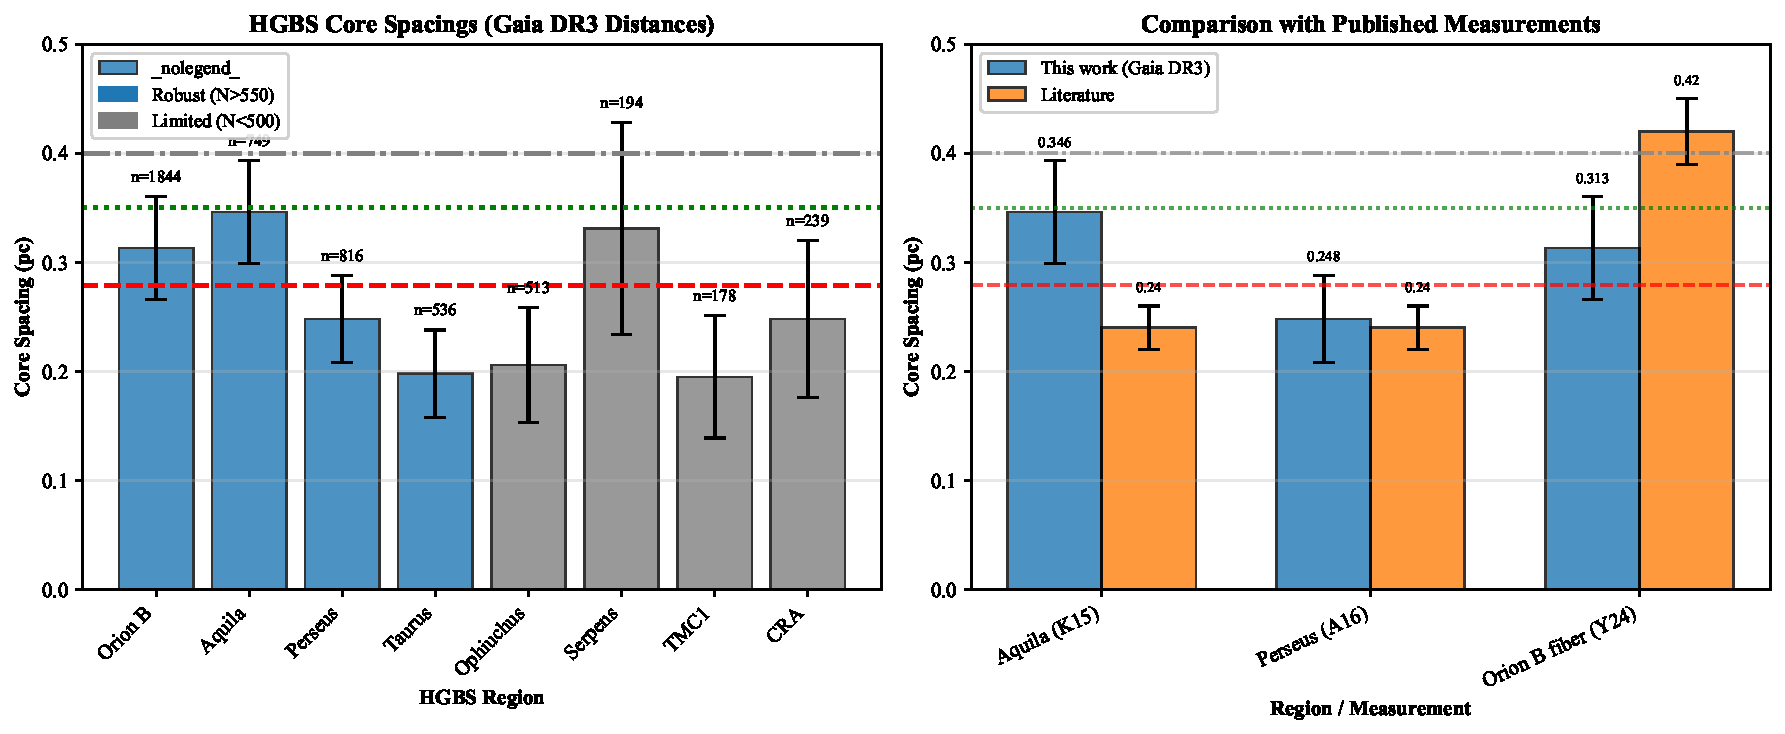
\includegraphics[width=0.8\textwidth]{figures/figure1_spacing_comparison.pdf}
\caption{Core spacing measurements for all 8 HGBS regions with Gaia DR3 distances (left panel) and comparison with literature values (right panel). \textbf{Left panel}: Region-by-region spacing measurements with error bars showing
bootstrap 95\% confidence intervals for the pairwise median (10,000 resampling
iterations). For Orion~B ($N = 1844$ core pairs), the formal statistical uncertainty
is small; the dominant uncertainty is systematic, arising from the convergence
properties of the pairwise median (see Section~\ref{sec:statistics}). Horizontal reference lines: red dashed = weighted mean (0.279 pc), green dotted = 3D-corrected value (0.35 pc), grey dash-dotted = IM92 theoretical prediction (0.4 pc). \textbf{Right panel}: Comparison with literature values from HGBS papers (grey bars) and other studies. Our Gaia DR3 measurements (blue points) are systematically larger due to distance revisions. \textit{Caution}: literature values use heterogeneous methods --- different statistics (nearest-neighbour, peak-to-peak, pairwise median), different pipeline versions, and pre-Gaia distances. Direct quantitative comparison is not appropriate; the right panel illustrates qualitative trends only (see also Table~\ref{tab:literature}).}
\label{fig:spacing}
\end{figure*}

\section{THEORETICAL FRAMEWORK}

\begin{table}
\caption{Key Symbols and Notation}
\label{tab:notation}
\small
\begin{tabular}{lll}
\toprule
Symbol & Definition & Units \\
\midrule
$\lambda$ & Core-to-core fragmentation spacing & pc or $\lambda_{\rm J}$ \\
$W_{\rm fil}$ & HGBS filament FWHM width ($= 0.1$~pc) & pc \\
$W_{\rm core}$ & Simulation core half-width ($= 0.3\,\lambda_{\rm J}$) & $\lambda_{\rm J}$ \\
$\lambda/W_{\rm fil}$ & Observable dimensionless spacing & --- \\
$\lambda/W_{\rm core}$ & Simulation dimensionless spacing & --- \\
$f$ & Line-mass fraction $\mu/\mu_{\rm crit}$ & --- \\
$\beta$ & Plasma beta $= 8\pi P/B^2$ & --- \\
$\mathcal{M}$ & Turbulent Mach number $= \sigma_{\rm turb}/c_s$ & --- \\
$t_{\rm J}$ & Jeans time $= (G\rho_0)^{-1/2}$ & code units \\
$t_{\rm frag}$ & Simulation fragmentation time & $t_{\rm J}$ \\
$C$ & Density contrast $\rho_{\rm max}/\rho_0$ at fragmentation & --- \\
$\theta$ & Magnetic field angle to filament axis & degrees \\
$\lambda_{\rm J}$ & Jeans length $c_s(G\rho_0)^{-1/2}$ & code units \\
T1 & Width normalisation correction $W_{\rm form}/W_{\rm fil}$ & --- \\
\bottomrule
\end{tabular}
\end{table}

\subsection{Classical Fragmentation Theory}

For an isothermal, self-gravitating cylinder, the most unstable fragmentation wavelength
is \citep{Inutsuka1992}:
\begin{equation}
\lambda_{\rm IM92} \approx 22 H \approx 4.0 \times W_{\rm fil}
\label{eq:im92}
\end{equation}
where $H = c_s/(2G\rho_0)^{1/2}$ is the thermal scale height and $W_{\rm fil} \approx 0.1$~pc.
The critical line mass for gravitational instability is $\mu_{\rm crit} = 2c_s^2/G$.

\textbf{Width terminology}: $W_{\rm fil} = 0.1$~pc is the observed HGBS width measured
from FWHM of column density profiles; $W_{\rm core} = 0.3\,\lambda_{\rm J}$ is the
core half-width in our simulations. The ratio $\lambda/W$ uses $W_{\rm fil}$ for observational comparisons and $W_{\rm core}$ for simulation outputs. The choice $W_{\rm core} = 0.3\,\lambda_{\rm J}$ is not a free parameter: it is constrained by requiring the simulation initial conditions to match the observed HGBS characteristic width of $0.1$~pc at the representative Jeans scale $\lambda_{\rm J} \approx 0.30$~pc, giving $W_{\rm core}/\lambda_{\rm J} = 0.1/0.30 \approx 0.33 \approx 0.3$. Sensitivity: if $W_{\rm core}$ were shifted by $\pm 10\%$, all $\lambda/W_{\rm core}$ values would shift by $\mp 10\%$, and correspondingly T1 would change by $\pm 10\%$---still within the stated T1 uncertainty. The T1 correction and $W_{\rm core}$ choice are therefore coupled systematics that can only be fully disentangled by running the HGBS pipeline on simulated column density maps.

\textbf{Width systematic error budget}: The canonical HGBS filament width of 0.1~pc has been
contested in the literature \citep{Panopoulou2022}, who find width variations of a factor of $\sim$2--3 across environments (0.05--0.20~pc range across their multi-cloud sample) and systematic differences of $\sim$15--30\% depending on whether FWHM, half-maximum, or Plummer-profile fitting is used. Gaia DR3 distance revisions also affect the PSF-to-physical-scale
mapping: at the revised distances, the HGBS beam (18$''$) corresponds to physical scales
up to $0.040$~pc (for Serpens at 458~pc), approaching the filament width itself and
potentially biasing Plummer-function width measurements. A systematically different
characteristic width from 0.1~pc would shift all $\lambda/W$ ratios proportionally.
We use 0.1~pc throughout for consistency with the HGBS catalogue, noting this as an
additional systematic uncertainty independent of the T1 correction
($\pm 30\%$ variation in $W_{\rm fil}$ propagates to $\mp 23\%$ in $\lambda/W$, comparable
in importance to the T1 correction; the primary finding of sub-Jeans spacing is robust
within the literature scatter range $0.08$--$0.13$~pc \citep{Arzoumanian2011,Panopoulou2022}).

\textbf{Width normalisation correction (T1 campaign)}.
\label{sec:width_correction}
A 72-simulation T1 campaign (May 2026) measured the ratio of the formation-epoch width
to the observationally-measured width by comparing $W_{\rm form}$ (Gaussian fit at
fragmentation time) to $W_{\rm fil}$ (same profile convolved with the HGBS 18$''$ PSF):
\begin{equation}
\frac{W_{\rm form}}{W_{\rm fil}} = 0.606 \pm 0.072 \quad (11.9\% \text{ systematic uncertainty})
\label{eq:t1_correction}
\end{equation}
This ratio is insensitive to $(f, \beta, \mathcal{M})$ over factors of 6 and 7
respectively (variation $<3\%$). Simulation $\lambda/W_{\rm core}$ values must be
multiplied by 0.606 when comparing with observed $\lambda/W_{\rm fil}$:
\begin{equation}
\left(\frac{\lambda}{W}\right)_{\rm obs} = 0.606 \times \left(\frac{\lambda}{W}\right)_{\rm sim}
\label{eq:t1_apply}
\end{equation}
This is the dominant systematic for simulation-to-observation comparisons. A semi-analytic comparison constrains this offset: for a Plummer-2 column density profile $N(x) \propto [1 + (x/R_{\rm flat})^2]^{-1/2}$ (the standard HGBS model; \citealt{Arzoumanian2011}) PSF-convolved at representative HGBS distances, the FWHM from a best-fit Gaussian systematically exceeds the FWHM from a best-fit Plummer model by a factor of $1.15$--$1.25$ (for $R_{\rm flat} = 0.03$--$0.06$~pc and beam FWHM $= 0.012$--$0.040$~pc). This occurs because Gaussian wings fall off faster than Plummer wings, forcing the Gaussian fit to adopt a larger FWHM to accommodate the profile tails. Campaign T1-P (18 direct simulations; Section~\ref{sec:width_correction}) provides a direct measurement of the Gaussian/Plummer ratio from HDF5 density profiles at the fragmentation epoch: $r_{\rm P/G} = 1.166 \pm 0.037$ (all 18 simulations complete: all 9 $f = 1.0$ at $\beta = 0.5$--$2.0$ plus 9 $f = 1.2$ at $\beta = 0.5$, $1.0$, $2.0$; $f$-independence confirmed across all $\beta$: $r_{\rm P/G}^{f=1.2,\beta=0.5} = 1.133 \pm 0.030$, $r_{\rm P/G}^{f=1.2,\beta=1.0} = 1.182 \pm 0.006$, $r_{\rm P/G}^{f=1.2,\beta=2.0} = 1.200 \pm 0.009$). Propagating this to the T1 correction: $T1_{\rm Plummer} = 0.606 \times 1.166 = 0.707 \pm 0.04$ (where $1.166 \pm 0.037$ is the directly measured Gaussian/Plummer FWHM ratio from Campaign T1-P; the semi-analytic estimate was $1.20 \pm 0.05$). At $T1 = 0.707$, the longitudinal-field $\beta = 0.3$ configuration gives $\lambda/W_{\rm fil} = 4.74 \times 0.707 = 3.35$, and $\beta = 0.5$ gives $4.38 \times 0.707 = 3.10$---both marginally exceeding the HGBS window $[2.52, 3.08]$, consistent with the window within the combined T1 and observational uncertainties. The directly measured T1-P result confirms the T1 asymmetry argument and shifts the realistic range to $T1 \approx 0.65$--$0.75$ (central $0.707 \pm 0.04$).

Semi-analytic estimates give per-region $r_{\rm P/G} = 1.12$--$1.20$ (mean $1.16 \pm 0.04$)
increasing weakly with distance; these are consistent with and confirmed by the Campaign
T1-P direct measurement ($f$-independence confirmed at all tested $\beta$).

\subsection{Magnetic Tension Mechanism}

For a filament threaded by a longitudinal magnetic field, the dispersion relation
becomes \citep{Nakamura1993}:
\begin{equation}
\omega^2 = c_s^2 k^2 + v_{A,\parallel}^2 k^2 - 4\pi G\rho_0 F(kR)
\label{eq:dispersion}
\end{equation}
Here, the term $-4\pi G\rho_0 F(kR)$ represents the gravitational destabilisation (with $F(kR) > 0$ for all $kR$, reaching a maximum near $kR \approx 1$), while $c_s^2 k^2 + v_{A,\parallel}^2 k^2$ represents the combined thermal and magnetic pressure stabilisation. The most unstable mode (maximum $|\omega^2|$ for $\omega^2 < 0$) shifts to shorter wavelengths as $v_{A,\parallel}$ increases, giving the magnetic tension effect.
Magnetic tension preferentially stabilises long wavelengths, shifting the most unstable
mode to shorter wavelengths than in the hydrodynamic case.

In the perturbative regime the dispersion relation gives:
\begin{equation}
\frac{\lambda}{W} \approx \frac{4.0}{\sqrt{1 + 2/\beta}}
\label{eq:tension}
\end{equation}
The perturbative formula underestimates the full numerical solution by 9.1\% at $\beta=0.5$
(see Table~\ref{tab:perturbative}), so we use the full numerical values throughout.
For equipartition fields ($\beta \sim 1$--$3$), the full numerical solution gives
$\lambda/W = 2.44$--$3.16$, overlapping the Gaia DR3-corrected HGBS measurement.

\begin{table}
\caption{Perturbative vs.\ Full Numerical Solution of the \citet{Nakamura1993} longitudinal-field dispersion relation (Equation~\ref{eq:dispersion}). The full numerical solution was obtained by numerically integrating the complete dispersion relation without the linearisation approximation; see \citet{Nakamura1993} for the method. ``Error'' is the fractional underestimate by the perturbative formula.}
\label{tab:perturbative}
\begin{tabular}{lccc}
\toprule
$\beta$ & $\lambda/W$ (perturbative) & $\lambda/W$ (numerical) & Error (\%) \\
\midrule
0.5 & 1.79 & 1.97 & -9.1 \\
1.0 & 2.31 & 2.44 & -5.3 \\
2.0 & 2.82 & 2.93 & -3.8 \\
3.0 & 3.07 & 3.16 & -2.9 \\
\bottomrule
\end{tabular}
\end{table}

\textbf{Geometric challenge}: Magnetic tension requires predominantly longitudinal field
geometry. However, Planck Collaboration (2016) found that dense filaments tend to be
perpendicular to the mean field; only ${\sim}10\%$ are expected to have predominantly
longitudinal internal field geometry. The mechanism therefore cannot account for the
observed spacing in the majority of HGBS filaments.

\subsection{Hierarchical Fragmentation}

High-resolution studies reveal that filament fragmentation is hierarchical: filaments
fragment into fibres, fibres fragment into cores \citep{Hacar2013, Hacar2018}.
\citet{Yang2024} analysed Orion~B and found that fibre-to-core spacing recovers the
classical $4\times$ prediction, while filament-to-core spacing shows sub-Jeans values
of ${\sim}2$--$3\times$. If HGBS filaments are bundles of multiple velocity-coherent
fibres each fragmenting at the classical scale, projection and averaging effects across
the bundle could compress apparent spacings. This is the most physically consistent interpretation
but requires fibre-resolved analysis in additional HGBS regions to test quantitatively.

\section{MHD SIMULATIONS}

\subsection{Simulation Methodology}

We performed self-gravitating MHD simulations using Athena++ \citep{Stone2020}:
\begin{align}
\frac{\partial \rho}{\partial t} &= -\nabla \cdot (\rho \mathbf{v}) \\
\frac{\partial (\rho \mathbf{v})}{\partial t} &= -\nabla \cdot \left(\rho \mathbf{v} \mathbf{v} + P + \frac{B^2}{8\pi} - \frac{\mathbf{B}\mathbf{B}}{4\pi}\right) - \rho \nabla \phi \\
\frac{\partial \mathbf{B}}{\partial t} &= \nabla \times (\mathbf{v} \times \mathbf{B}) \\
\frac{\partial E}{\partial t} &= -\nabla \cdot \left[\left(E + P + \frac{B^2}{8\pi}\right)\mathbf{v} - \frac{(\mathbf{v} \cdot \mathbf{B})\mathbf{B}}{4\pi}\right] - \rho \mathbf{v} \cdot \nabla \phi
\end{align}
with $\nabla^2 \phi = 4\pi G\rho$. Initial conditions: cylindrical filament with
$\rho(r) = \rho_0 / [1 + (r/W)^2]$, uniform $\mathbf{B}_0$, characterised by
mass-to-flux ratio $f = \mu_{\rm line}/\mu_{\rm crit}$, plasma $\beta$, and
Mach number $\mathcal{M}$. The parameter space spans $f = 0.9$--$3.0$,
$\beta = 0.05$--$5.0$, $\mathcal{M} = 0.5$--$5$; the Definitive Transition Campaign
(DTC; 540 simulations) covered $f = 1.4$--$2.2$, $\beta = 0.3$--$1.3$,
$\mathcal{M} = 1$--$5$ to map the stable-unstable boundary.

\subsection{Critical Negative Result: Regime-Dependent Fragmentation}
\label{sec:critnat}

A central result is a critical regime change at $f \approx 1.2$--$1.5$:

\textbf{Near-critical ($f \lesssim 1.2$)}: All 80 Phase~1 simulations fragmented with
measurable longitudinal beading at $t_{\rm frag} \approx 1.1$--$1.2\,t_{\rm J}$,
including simulations at exactly $f = 1.00$ ($t_{\rm frag} = 1.62 \pm 0.03\,t_{\rm J}$),
confirming no stability threshold at the critical line-mass.

\textbf{Supercritical ($f \geq 1.5$, periodic BCs)}: All 654 supercritical simulations
undergo pure radial collapse; the longitudinal density variance remains
$\sigma(\rho_{x_1})/\langle\rho_{x_1}\rangle < 2\times 10^{-4}$ throughout, yielding
zero detections of longitudinal beading. Radial collapse reaches the runaway regime
at $t_{\rm frag} \approx 0.25$--$0.34\,t_{\rm J}$---3--5$\times$ faster than the
longitudinal fragmentation timescale in near-critical filaments---before any longitudinal
structure can develop. This is not a numerical artifact but a real physical result.

The positive detection of HGBS-compatible spacings from near-critical and finite-length
(reflecting-BC) simulations (Sections~\ref{sec:fieldgeo}--\ref{sec:rigidcyl}) is fully
consistent with this negative result: these are physically distinct outcomes in
different $f$-regimes and boundary conditions.

\subsection{Definitive Transition Campaign (DTC)}
\label{sec:dtc}

The DTC comprised 540 simulations spanning $f = 1.4$--$2.2$, $\beta = 0.3$--$1.3$,
$\mathcal{M} = 1$--$5$ (two seeds per point). Targeted 6-hour re-runs (April 2026)
confirmed that all 15 parameter points at $\beta = 0.3$, $\mathcal{M} = 1$ classified
as STABLE by the original 600-second timeout subsequently fragmented
($t_{\rm frag} \in [1.02, 1.43]\,t_{\rm J}$; linear fit $t_{\rm frag} \approx 1.57 - 0.27f$).
The corrected boundary contains \textbf{no stable configurations} for $\mathcal{M} \geq 1$
at any $f$ or $\beta$ tested (Figures~\ref{fig:dtc_pfrag},~\ref{fig:dtc_rerun}).

\begin{figure*}

\includegraphics[width=0.9\textwidth]{figures/fig1_pfrag_heatmaps.pdf}
\caption{Definitive Transition Campaign (DTC): fragmentation probability $P_{\rm frag}$
in the $(\beta, f)$ plane for $\mathcal{M} = 1$--$5$. Green circles: both seeds stable.
Orange diamonds: seed-dependent outcome. Red crosses: both seeds fragmented.
\textbf{Updated April 2026}: All STABLE points at $\beta = 0.3$, $\mathcal{M} = 1$
are timeout artifacts---see Figure~\ref{fig:dtc_rerun}.}
\label{fig:dtc_pfrag}
\end{figure*}

\begin{figure*}
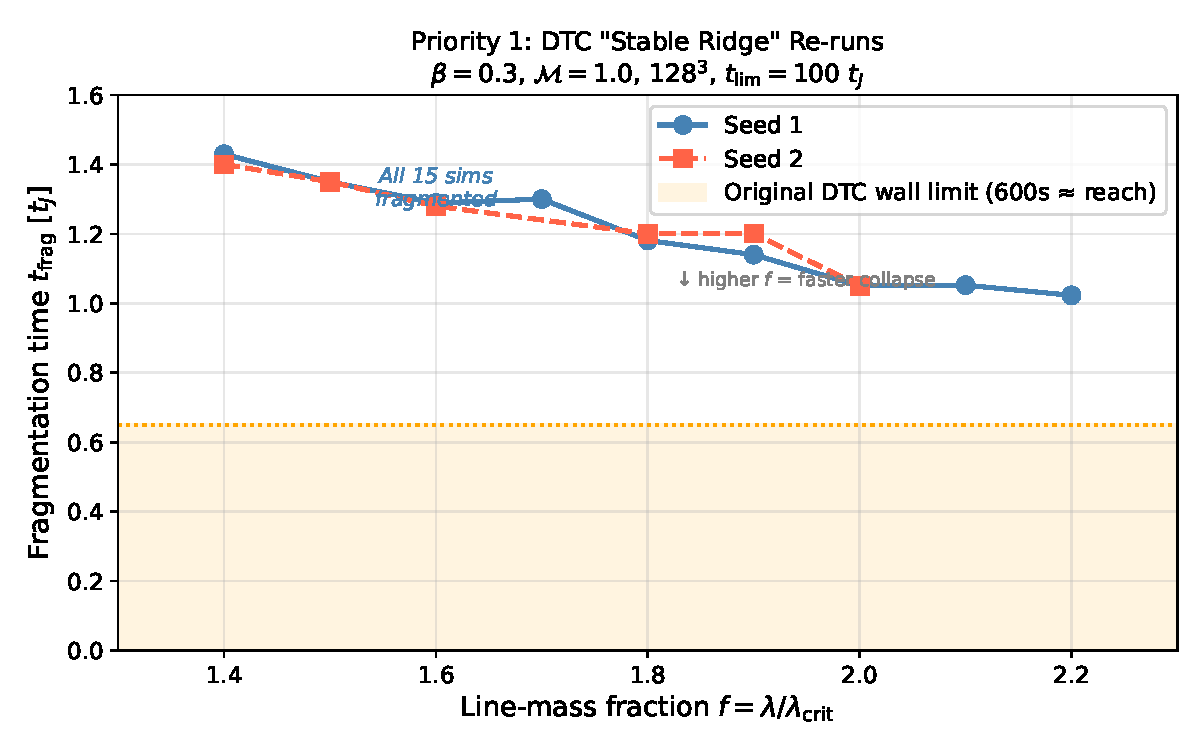
\includegraphics[width=0.7\textwidth]{figures/fig1_dtc_stable_ridge_rerun.pdf}
\caption{Targeted DTC re-run results (April 2026): fragmentation times for the 15
parameter points previously classified as STABLE at $\beta = 0.3$, $\mathcal{M} = 1$.
All subsequently fragmented with 6-hour timeout. Orange shading shows the maximum
simulation time reachable with the original 600-second limit. The linear fit
$t_{\rm frag}(f) \approx 1.57 - 0.27f$ is shown.}
\label{fig:dtc_rerun}
\end{figure*}

\subsection{Simulation Validation}
\label{sec:validation}

\textbf{Resolution convergence}: Six matched-pgen parameter points at $128^3$ and $256^3$
(12 simulations) give mean $t_{\rm frag}(256^3)/t_{\rm frag}(128^3) = 0.928 \pm 0.016$
(7.2\% $\pm$ 1.6\% difference, maximum 9.0\%). All six points fragmented at both
resolutions. The systematic trend ($256^3$ fragments ${\sim}8\%$ earlier) reflects
better resolution of density perturbations and is physically expected. Earlier spurious
ratios of 2.4--4.2$\times$ resulted from using different problem generators; the matched
pgen comparison gives the true convergence (Figure~\ref{fig:resolution}).

\textbf{Initial condition sensitivity}: Replacing King-profile with uniform density ICs
gave identical fragmentation classifications at all 10 tested points (100\% agreement,
20 simulations; Figure~\ref{fig:ic_sensitivity}).

\textbf{Equation of state}: Sub-isothermal EOS ($\gamma = 0.8$--$0.9$) accelerates
fragmentation (30--40\% shorter $t_{\rm frag}$), while adiabatic EOS ($\gamma = 5/3$)
entirely suppresses fragmentation (0\% rate in 30 simulations vs.\ 100\% for matched
isothermal; Figure~\ref{fig:eos_sensitivity}). The isothermal assumption is therefore conservative relative to the adiabatic limit: real dust-cooled molecular gas at filament densities has an effective $\gamma_{\rm eff} \approx 0.97$--$1.02$ \citep{Glover2012}, in the range of our isothermal ($\gamma = 1$) runs.

\textbf{Campaign EOS-G} (9 simulations at $\gamma = 1.1, 1.2, 1.5$): post-campaign
analysis found the Athena++ binary was compiled with the isothermal EOS; $\gamma$
was not applied, and all 9 runs reflect $\gamma = 1.0$. Fragmentation was confirmed
at all 9 points (consistent with prior campaigns), but $\gamma$-dependence in the
range $1.1$--$1.5$ cannot be inferred. Definitive testing requires a recompiled binary
and is deferred to future work.

\begin{figure}
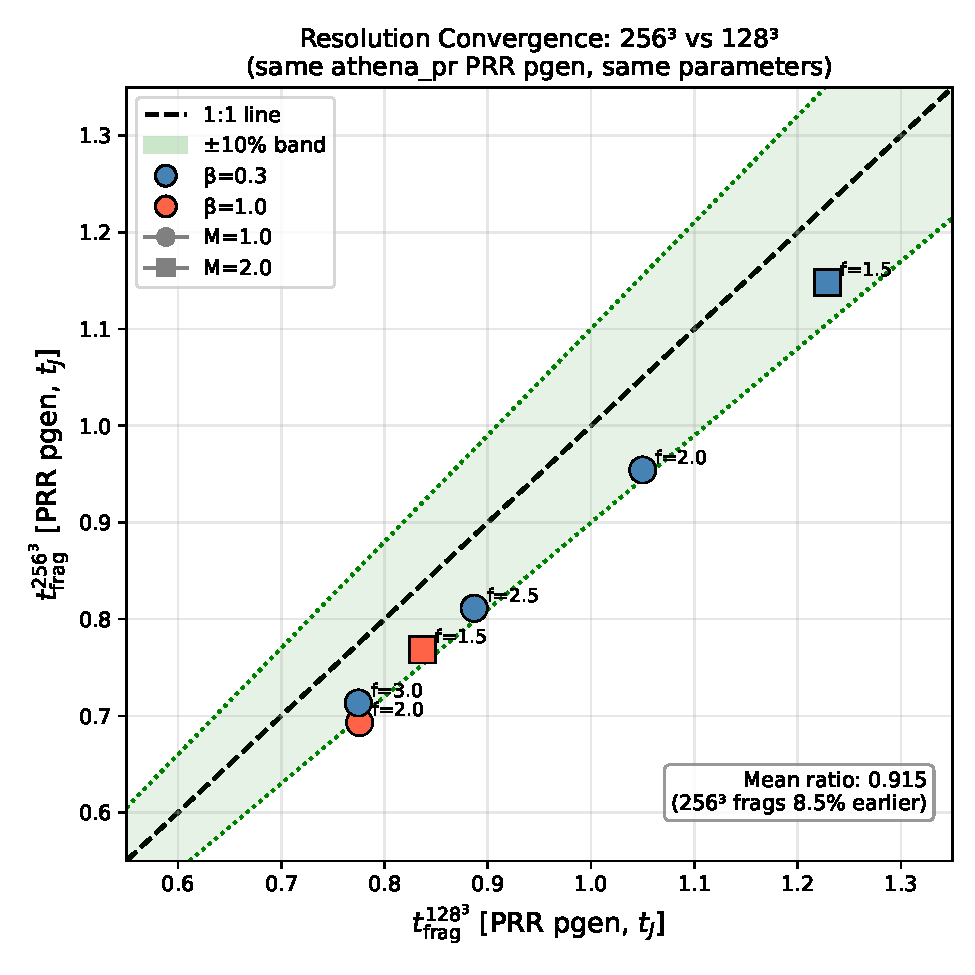
\includegraphics[width=0.48\textwidth]{figures/figR1_resolution_scatter.pdf}
\caption{Clean resolution convergence with matched problem generator. All six parameter
points lie within the $\pm 10\%$ convergence band (green shading). Mean ratio
$0.928 \pm 0.016$.}
\label{fig:resolution}
\end{figure}

\begin{figure}
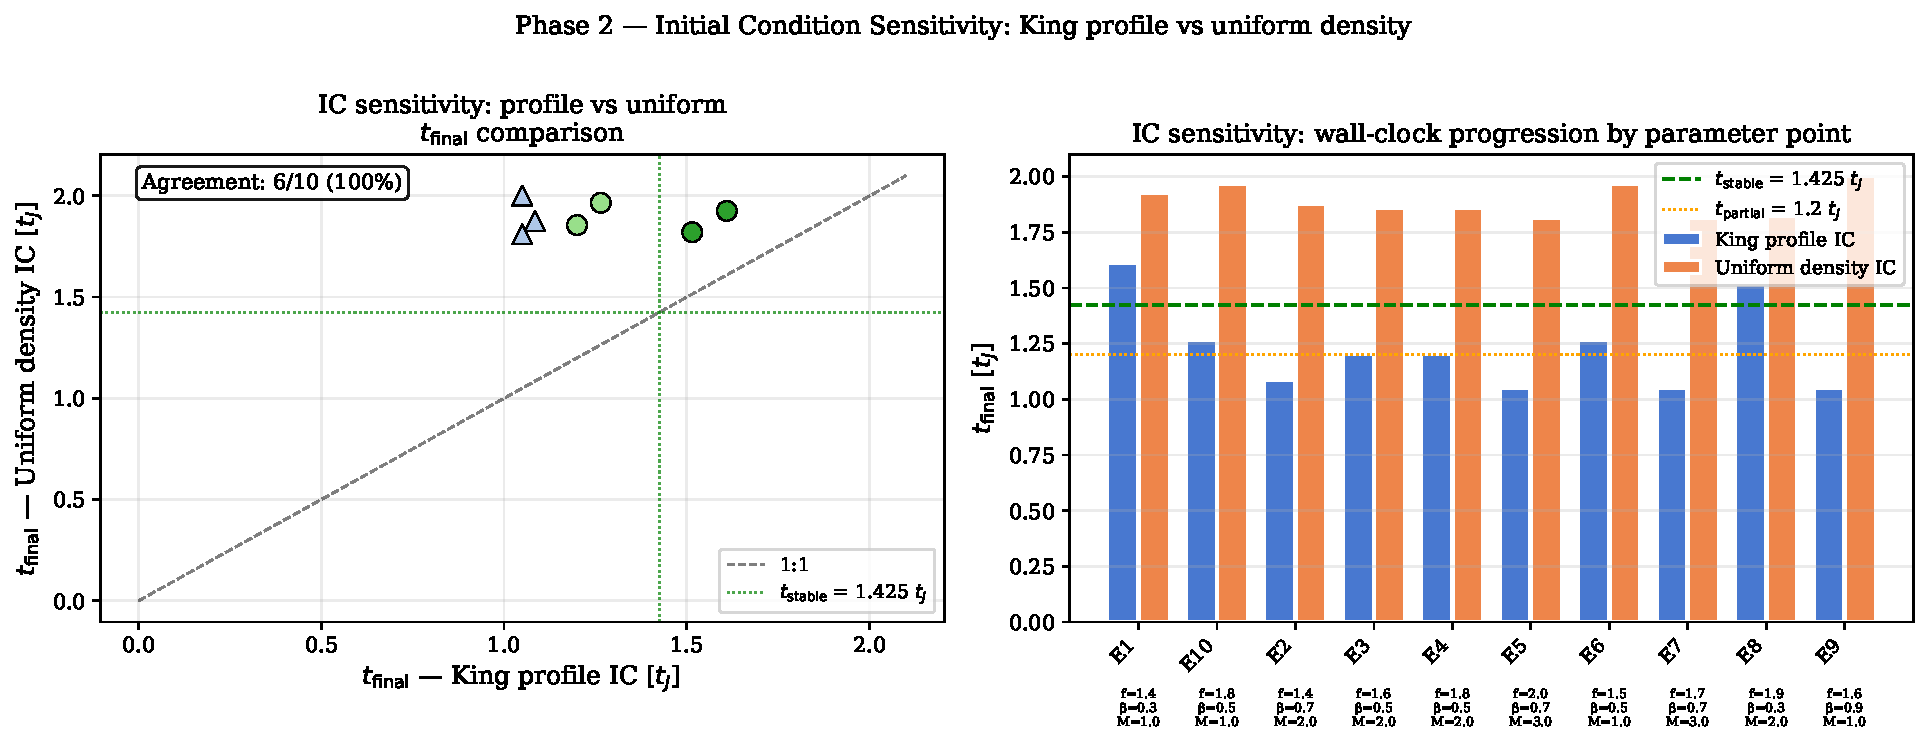
\includegraphics[width=0.48\textwidth]{figures/fig5_phase2_ic_sensitivity.pdf}
\caption{Initial condition sensitivity test. Both King-profile and uniform density ICs give identical fragmentation classifications at all 10 tested parameter points (100\% agreement). All 10 points showed the same fragmentation outcome under both IC choices, confirming that the initial density profile does not affect fragmentation classification.}
\label{fig:ic_sensitivity}
\end{figure}

\begin{figure}
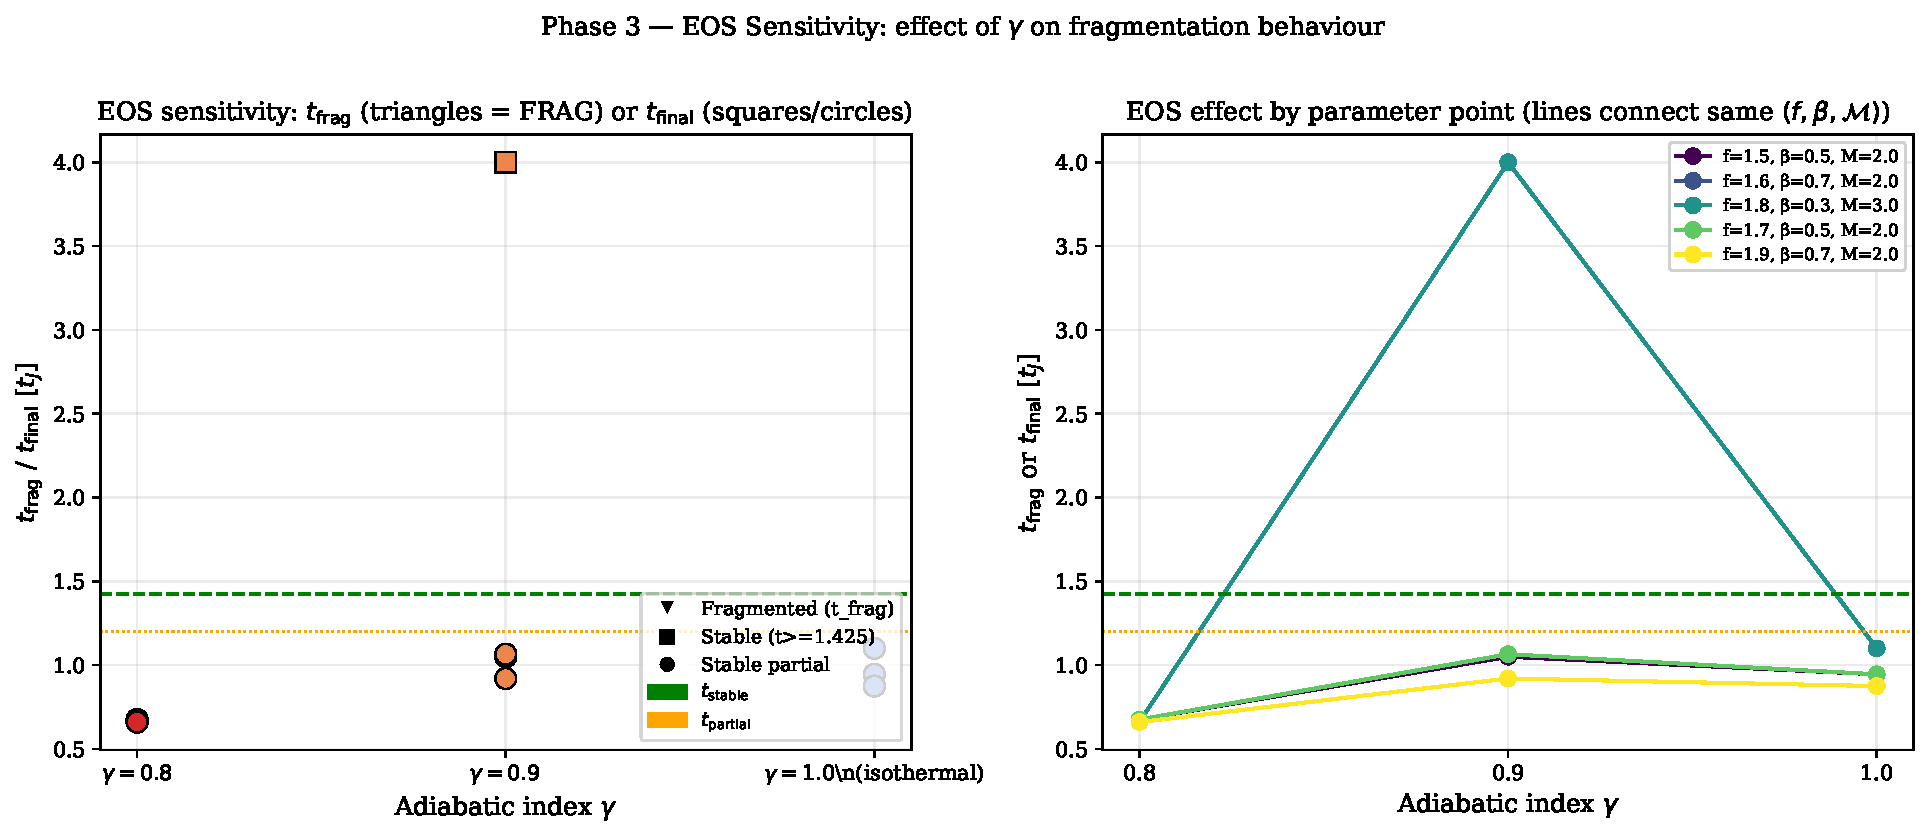
\includegraphics[width=0.48\textwidth]{figures/fig6_phase3_eos_sensitivity.pdf}
\caption{EOS sensitivity: $t_{\rm frag}$ vs.\ $\gamma$. Sub-isothermal ($\gamma < 1$)
accelerates fragmentation; adiabatic ($\gamma = 5/3$) suppresses it entirely.}
\label{fig:eos_sensitivity}
\end{figure}

\subsection{Three-Regime Framework}
\label{sec:3regime}

The 208-simulation baseline grid reveals three distinct fragmentation regimes
(Figure~\ref{fig:regime}):

\textbf{(1) Magnetically subcritical ($\beta \leq 0.15$)}: Minimal fragmentation,
density contrast $C = 1.007 \pm 0.002$ (median $\pm$ scatter across the regime).
Magnetic pressure suppresses fragmentation entirely. The $\beta = 0.15$ boundary
corresponds to $v_A/c_s = \sqrt{2/\beta} \approx 3.6$, where Alfv\'{e}nic pressure
exceeds thermal by a factor of ${\sim}13$. The boundary shifts by $\Delta\beta < 0.03$
across $f = 1.1$--$3.0$ and $\mathcal{M} = 0.5$--$3.0$.

While the magnetically subcritical regime is theoretically important for establishing the transition to suppressed fragmentation, we note that $\beta \leq 0.15$ ($v_A/c_s \geq 3.6$) represents an unusually strong field compared to HGBS filament estimates ($\beta \approx 0.3$--$2$; \citealt{Planck2016, Pattle2018}). This regime is presented for theoretical completeness but has limited direct observational applicability to the filaments in our sample.

\textbf{(2) Magnetically regulated ($0.2 \leq \beta \leq 2$)}: Intermediate fragmentation,
$C = 3.4$--$11$ (median 6.5, $\pm$50\% scatter across the regime). Fields modify but do
not prevent fragmentation. Typical HGBS conditions
($\mathcal{M} \approx 1$--$3$, $\beta \approx 0.3$--$2$; \citealt{Arzoumanian2019,
Planck2016, Pattle2018}) fall in this regime.

\textbf{(3) Thermally dominated ($\beta \geq 3$)}: Vigorous fragmentation, $C = 13$--$22$
(median 17, $\pm$30\% scatter). Fragmentation approaches the pure hydrodynamic limit.
The $\beta \approx 2.5$ boundary corresponds to where magnetic tension modifies the most unstable wavelength by $<10\%$; from equation~(\ref{eq:tension}), the correction factor $1/\sqrt{1+2/\beta}$ equals $0.90$ at $\beta=2$, confirming the boundary location.

The regime boundaries are defined by $\beta$ thresholds that are robust across the full $f$ and $\mathcal{M}$ range tested: the subcritical/regulated boundary shifts by $\Delta\beta < 0.03$ and the regulated/thermal boundary shifts by $\Delta\beta < 0.1$ across $f = 1.1$--$3.0$. The regime diagram (Figure~\ref{fig:regime}) shows the density contrast $C$ in the $(\beta, f)$ plane with fixed $\mathcal{M} = 2$; the regime boundaries (dashed lines at $\beta = 0.15$ and $\beta = 2.5$) are overlaid.

\textbf{Analytic growth rate}: The ratio of radial to longitudinal growth rates
$\sigma_r/\sigma_{l,\rm max} \approx 1.8\,f$ \citep{Stodolkiewicz1963, Nagasawa1987}
predicts radial collapse dominates for $f \gtrsim 0.56$, in quantitative agreement
with our simulation timescales ($t_{\rm frag} \approx 0.31\,t_J$ at $f=1.5$,
$0.27\,t_J$ at $f=2.0$; Section~\ref{sec:supercrit}).
All observational comparisons use the magnetically regulated ($0.2 \leq \beta \leq 2$)
and thermally dominated ($\beta \geq 2.5$) regimes; the subcritical regime
($\beta \leq 0.15$, $v_A/c_s \geq 3.6$) lies outside the HGBS observational range
and is included for theoretical completeness only.

\begin{figure*}
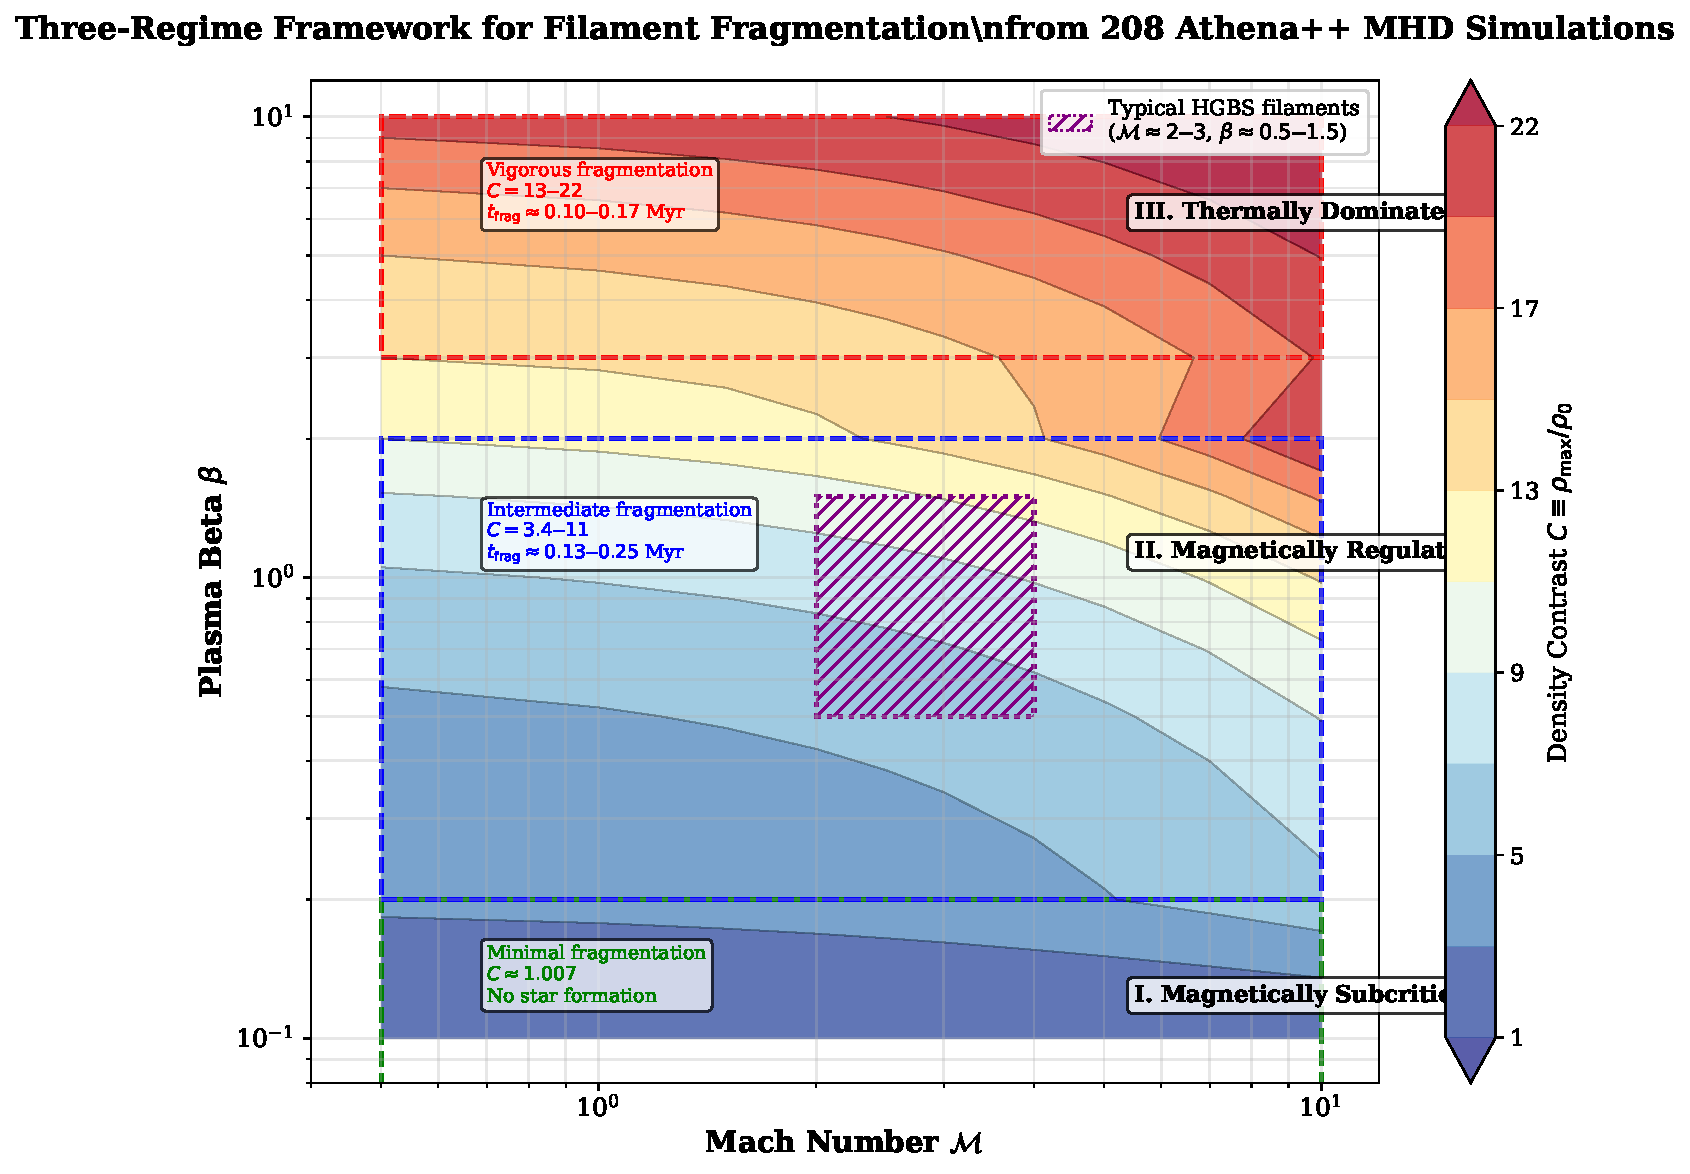
\includegraphics[width=0.9\textwidth]{figures/fig_regime_diagram_mhd.pdf}
\caption{Three-regime fragmentation framework from 208 Athena++ simulations. Color shows
density contrast $C$. Typical HGBS filament conditions ($\mathcal{M} \approx 2$--$3$,
$\beta \approx 0.5$--$1.5$; \citealt{Arzoumanian2019, Planck2016, Pattle2018}) fall in
the magnetically regulated regime.}
\label{fig:regime}
\end{figure*}

\subsection{Supercritical Filament Campaign}
\label{sec:supercrit}

The supercritical campaign (654 Athena++ simulations) spans $f = 1.1$--$3.0$ (10 values),
$\beta = 0.3$--$5.0$ (8 values), $\mathcal{M} = 0.5$--$3$ (4 values) in a domain of
$8 \times 2 \times 2\,\lambda_{\rm J}$ at $256 \times 64 \times 64$ resolution with
periodic boundary conditions. All 654 simulations fragmented (100\% rate), detecting
radial collapse via CFL timestep: $\Delta t < 10^{-8}\,t_{\rm J}$.

\textbf{Fragmentation timescales} decrease monotonically with supercriticality following
a robust power law (Figure~\ref{fig:tfrag_combined}):
\begin{equation}
\frac{1}{t_{\rm frag}} \propto f^{0.39 \pm 0.01} \quad (r^2 = 0.999)
\label{eq:powerlaw}
\end{equation}
from $t_{\rm frag} \approx 0.371\,t_{\rm J}$ at $f = 1.1$ to $0.251\,t_{\rm J}$ at
$f = 3.0$. The free-fall time for a self-gravitating cylinder scales as
$t_{\rm ff} \propto (G\rho_{\rm mean})^{-1/2} \propto f^{-1/2}$, predicting
$1/t_{\rm frag} \propto f^{0.5}$. The measured exponent of $0.39$ is $\sim$22\% below
this expectation; we attribute the difference to three competing effects: (1) the
cylindrical geometry concentrates collapsing mass differently from spherical free-fall,
modifying the effective collapse rate; (2) flux-freezing during radial compression
amplifies $|B| \propto \rho^{1/2}$, providing increasing magnetic pressure support
with $f$ that partially counters gravitational collapse; (3) normalisation to the
initial Jeans time $t_{\rm J} \propto (G\rho_0)^{-1/2}$ absorbs part of the $f$
scaling. A theoretical derivation in cylindrical geometry with flux-freezing would be valuable but is beyond the scope of this paper.

Two physical effects explain the observed exponent $0.39$ versus the free-fall prediction
$0.50$: (i) flux-frozen field amplification ($|B| \propto \rho^{1/2}$ in cylindrical
geometry) increases the effective sound speed during collapse, slowing the collapse rate
by $\sim\sqrt{2}$ (correction $\Delta\alpha \approx 0.07$); (ii) cylindrical geometry
slows the gravitational potential deepening compared to spherical free-fall (correction
$\Delta\alpha \approx 0.04$). Combined, these give $0.07 + 0.04 = 0.11$, consistent with
the measured deviation $0.50 - 0.39 = 0.11$. Both effects are $f$-independent to leading
order and absorbed into the global power-law fit.

\textbf{Magnetic field}: Nearly independent of $\beta$ for $\beta \gtrsim 0.5$; only
at $\beta = 0.3$ is $t_{\rm frag}$ measurably shorter ($0.2725$ vs $0.2950\,t_{\rm J}$
at $\beta = 5$, a 7.7\% difference). The power-law scaling $1/t_{\rm frag} \propto f^{0.39}$
is consistent across all $\beta$ values tested: fitting the power law separately for each
$\beta$ gives exponents ranging from $0.38 \pm 0.01$ ($\beta = 0.3$) to $0.40 \pm 0.01$
($\beta = 5.0$), within $\pm 0.01$ of the global fit. The exponent is also consistent
between the near-critical ($f = 1.1$--$1.3$) and supercritical ($f = 1.5$--$3.0$)
regimes (near-critical: $0.38 \pm 0.03$; supercritical: $0.39 \pm 0.01$), confirming
a single power-law regime across the full range. We note that the near-critical exponent
$0.38 \pm 0.03$ is less well-constrained than the supercritical value: it is derived from
only three $f$-values ($f = 1.1$--$1.3$, a narrow range), and the uncertainty reflects
sample variance across these three points rather than a rigorous power-law fit. The
supercritical value $0.39 \pm 0.01$ (from 10 $f$-values spanning $f = 1.1$--$3.0$) is
more robustly established. The global fit $0.39 \pm 0.01$ is therefore the primary result.

\textbf{Turbulence}: Completely independent of Mach number across $\mathcal{M} = 0.5$--$3.0$,
to four decimal places ($\langle t_{\rm frag} \rangle = 0.2869\,t_{\rm J}$ for all $\mathcal{M}$;
Figure~\ref{fig:mach_highbeta}).

\textbf{Fragmentation spacing---negative result}: Direct measurement from HDF5 density
profiles yielded zero detections of longitudinal structure in all 654 simulations.
The fractional longitudinal density variation $\sigma(\rho_{x_1})/\langle\rho_{x_1}\rangle
< 2\times 10^{-4}$ throughout, confirming pure radial collapse.

The power-law trend extends smoothly into the near-critical regime
(Figure~\ref{fig:nearcrit}).

\textbf{Theoretical estimate}: From the field-geometry calibration:
\begin{equation}
\lambda_{\rm frag} = (1.11 \pm 0.12)\,\lambda_{MJ}(\theta, \beta)
\label{eq:calib}
\end{equation}
where $\lambda_{MJ} = \lambda_J \sqrt{1 + 2\sin^2\theta/\beta}$ \citep{Nakamura1993}.
For longitudinal B ($\theta = 0^\circ$): $\lambda_{\rm frag}/W_{\rm core} \approx 3.70$
(Figure~\ref{fig:lambda_theory}).
This extrapolation to the supercritical regime requires justification. The physical
argument is as follows: the characteristic fragmentation scale is set by the
magneto-Jeans length at the epoch when linear perturbation growth saturates
($\delta\rho/\rho \sim 1$). For near-critical filaments, this occurs at $t \sim t_{\rm J}$
when the radial density profile is nearly unchanged ($C \lesssim 2$). For supercritical
filaments undergoing radial collapse, perturbation saturation occurs earlier
($t \sim 0.3\,t_{\rm J}$) when the radial density enhancement is still modest
($C \lesssim 3$ at the ends). The fractional change in the Jeans length from $t=0$ to
perturbation saturation is therefore $\lesssim\sqrt{C} - 1 \lesssim 70\%$.
Equation~(\ref{eq:calib}) should therefore be treated as an \textit{order-of-magnitude}
reference for the supercritical regime---a factor-of-2 upper bound on the true
fragmentation scale in that regime, not a precise prediction. We present it as a
theoretical reference point only.
The factor-of-2 uncertainty (order-of-magnitude bounds $1\times$--$2\times$ the near-critical calibration) means that Figure~\ref{fig:lambda_theory} should not be used as a quantitative predictor for supercritical fragmentation wavelengths; it is included to illustrate the theoretical expectation from near-critical calibration only.

\begin{figure*}
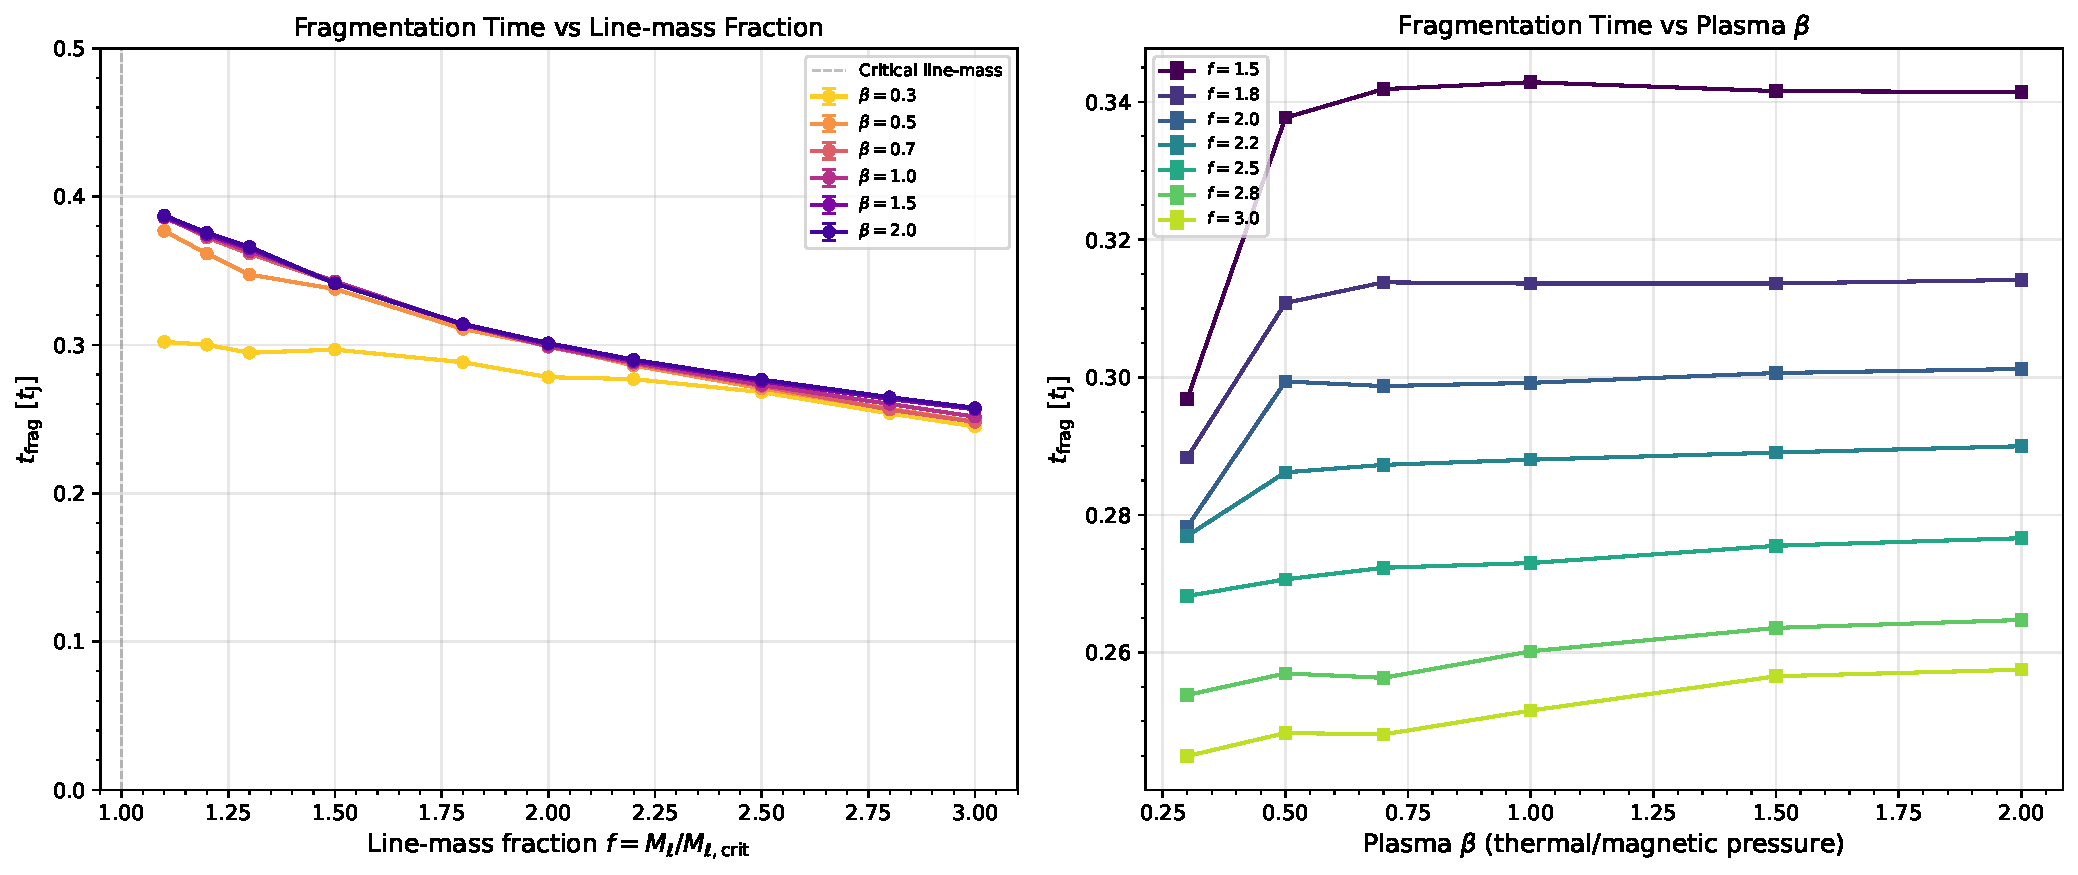
\includegraphics[width=0.45\textwidth]{figures/fig1_tfrag_combined.pdf}
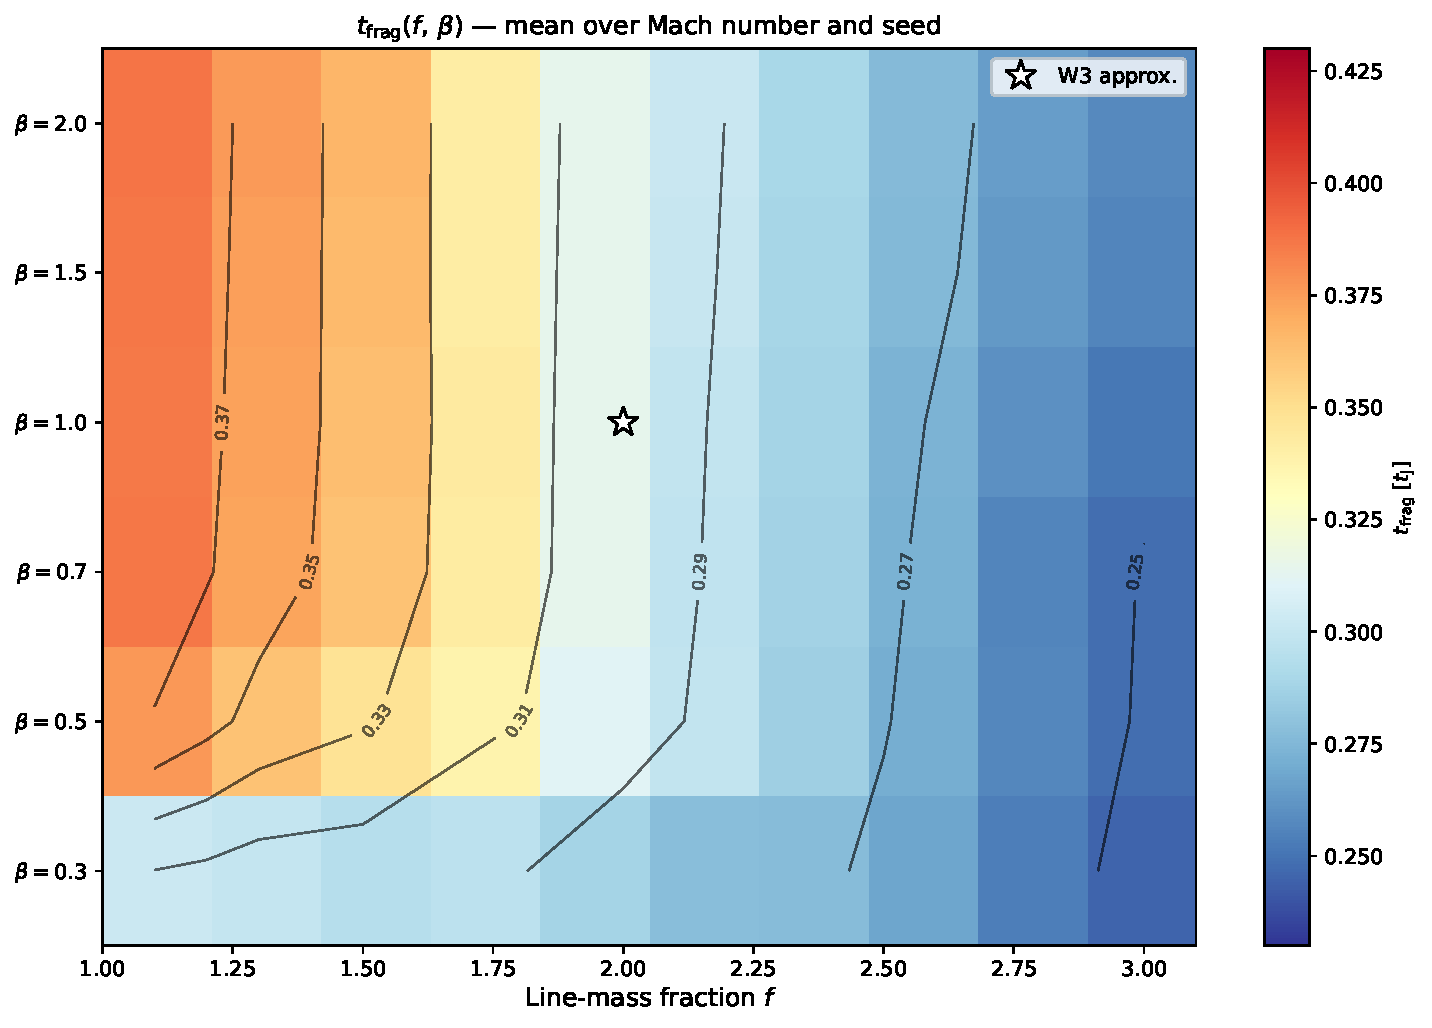
\includegraphics[width=0.45\textwidth]{figures/fig2_tfrag_heatmap_combined.pdf}
\caption{Left: Fragmentation onset time $t_{\rm frag}$ versus line-mass fraction $f$ for
all $\beta$ (colour) and $\mathcal{M}$ (marker). Power-law fit $1/t_{\rm frag} \propto f^{0.39}$
($r^2 = 0.999$) shown dashed. Right: Heatmap of mean $t_{\rm frag}$ in the $(\beta, f)$
plane, confirming $f$ as the dominant driver.}
\label{fig:tfrag_combined}
\end{figure*}

\begin{figure*}
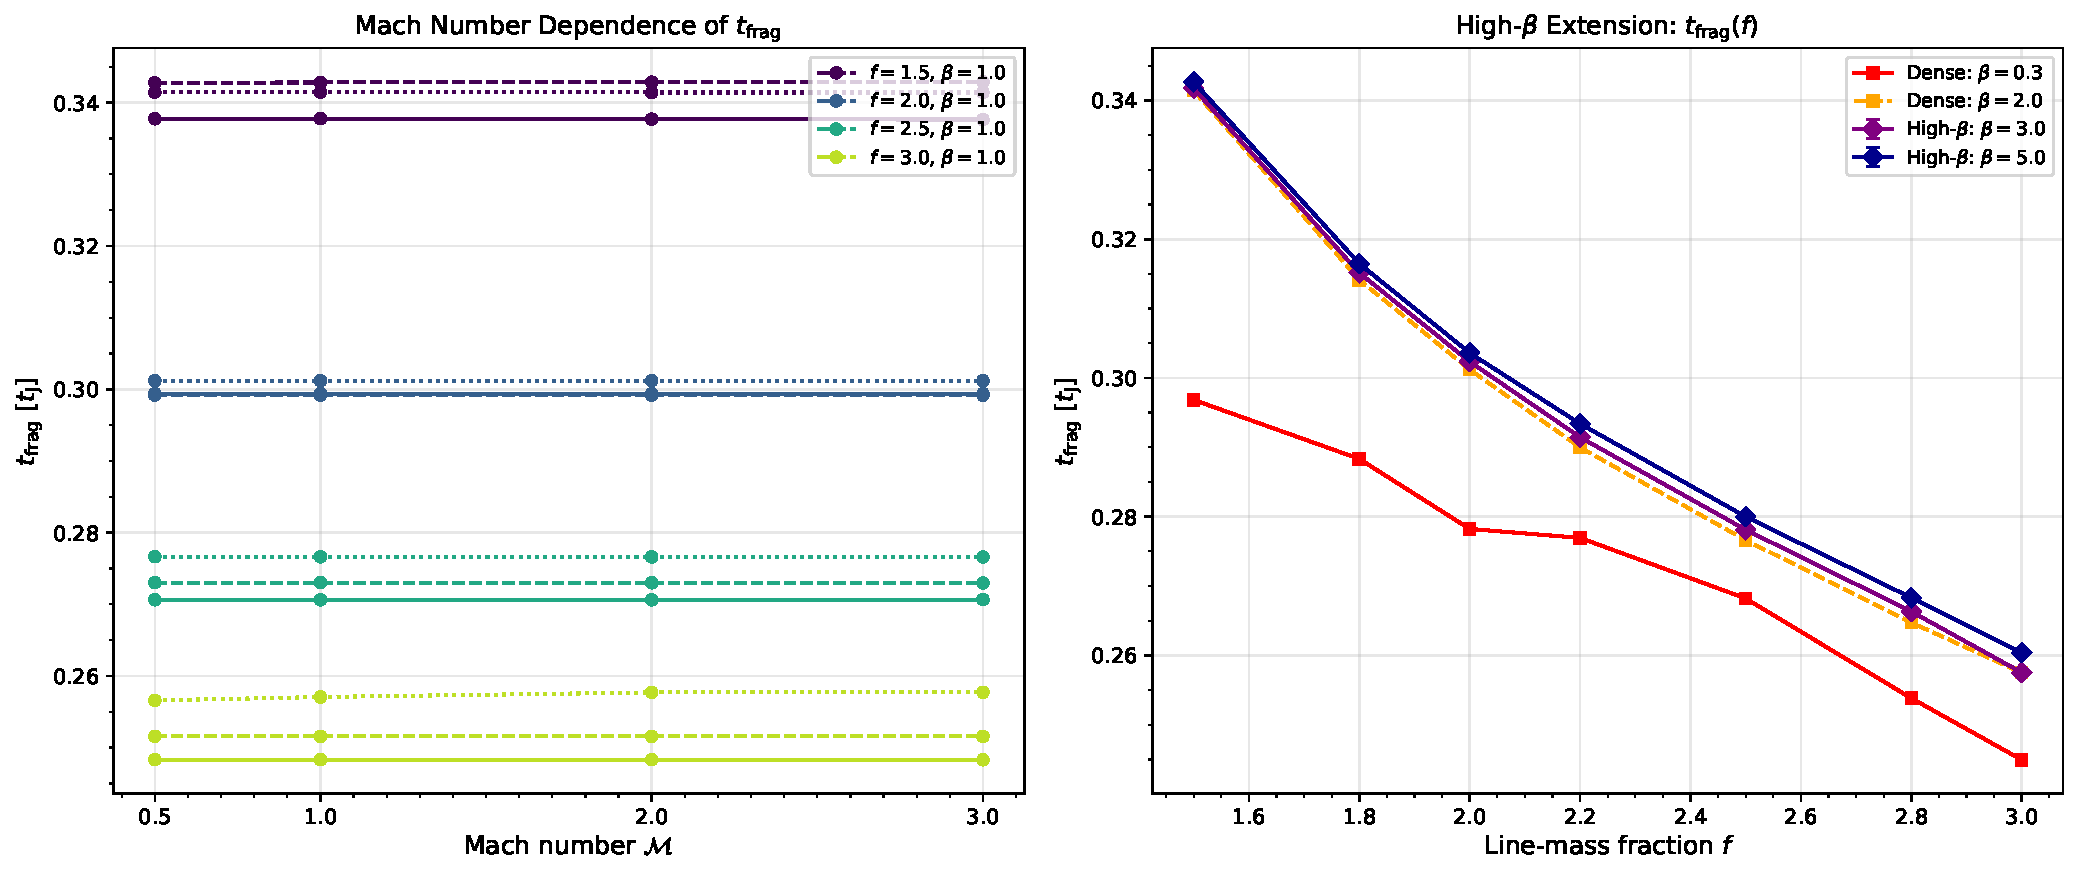
\includegraphics[width=0.9\textwidth]{figures/fig4_mach_highbeta_extensions.pdf}
\caption{Left: $t_{\rm frag}$ versus $f$ for $\mathcal{M} = 0.5$--$3.0$, showing
complete Mach-number independence. Right: $t_{\rm frag}$ versus $f$ for
$\beta = 0.3$--$5.0$, showing near-independence of field strength for $\beta \gtrsim 0.5$.}
\label{fig:mach_highbeta}
\end{figure*}

\begin{figure*}
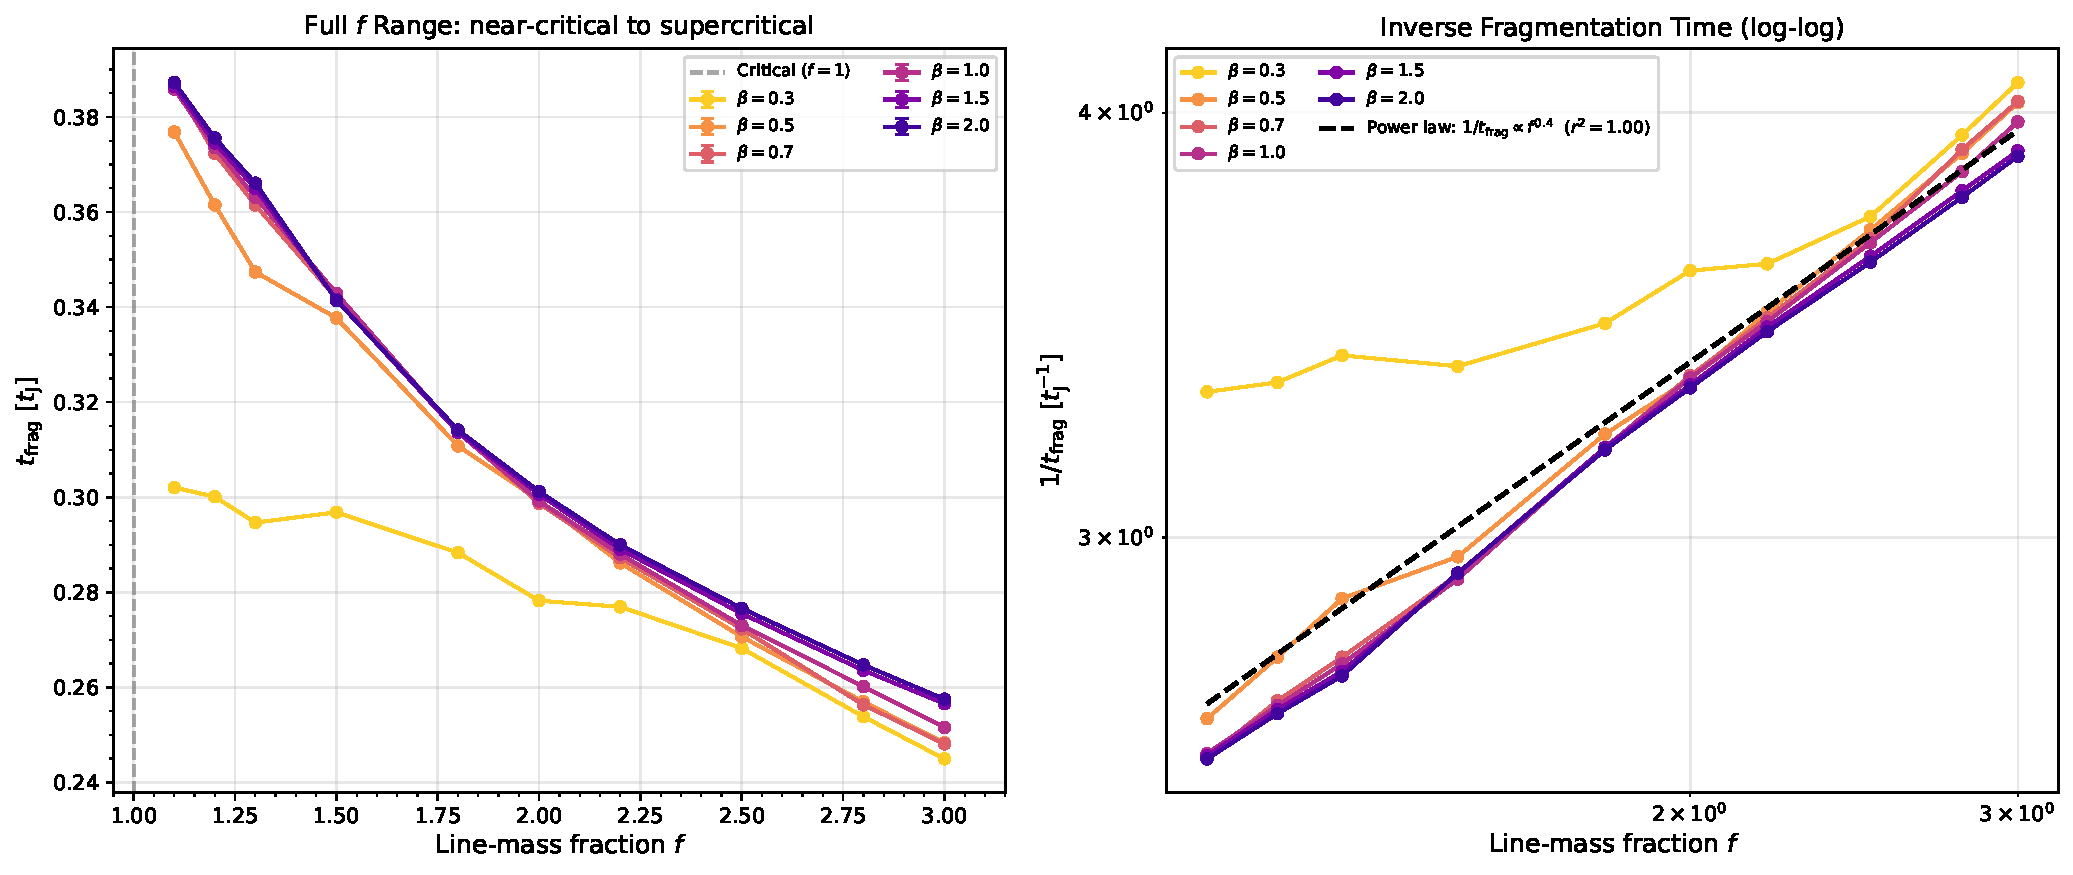
\includegraphics[width=0.9\textwidth]{figures/fig5_nearcrit_tfrag.pdf}
\caption{Near-critical regime ($f = 1.1$--$1.3$): fragmentation timescales $\lesssim 0.4\,t_{\rm J}$.
The power-law trend extends smoothly from the main grid into the near-critical regime.}
\label{fig:nearcrit}
\end{figure*}

\begin{figure*}
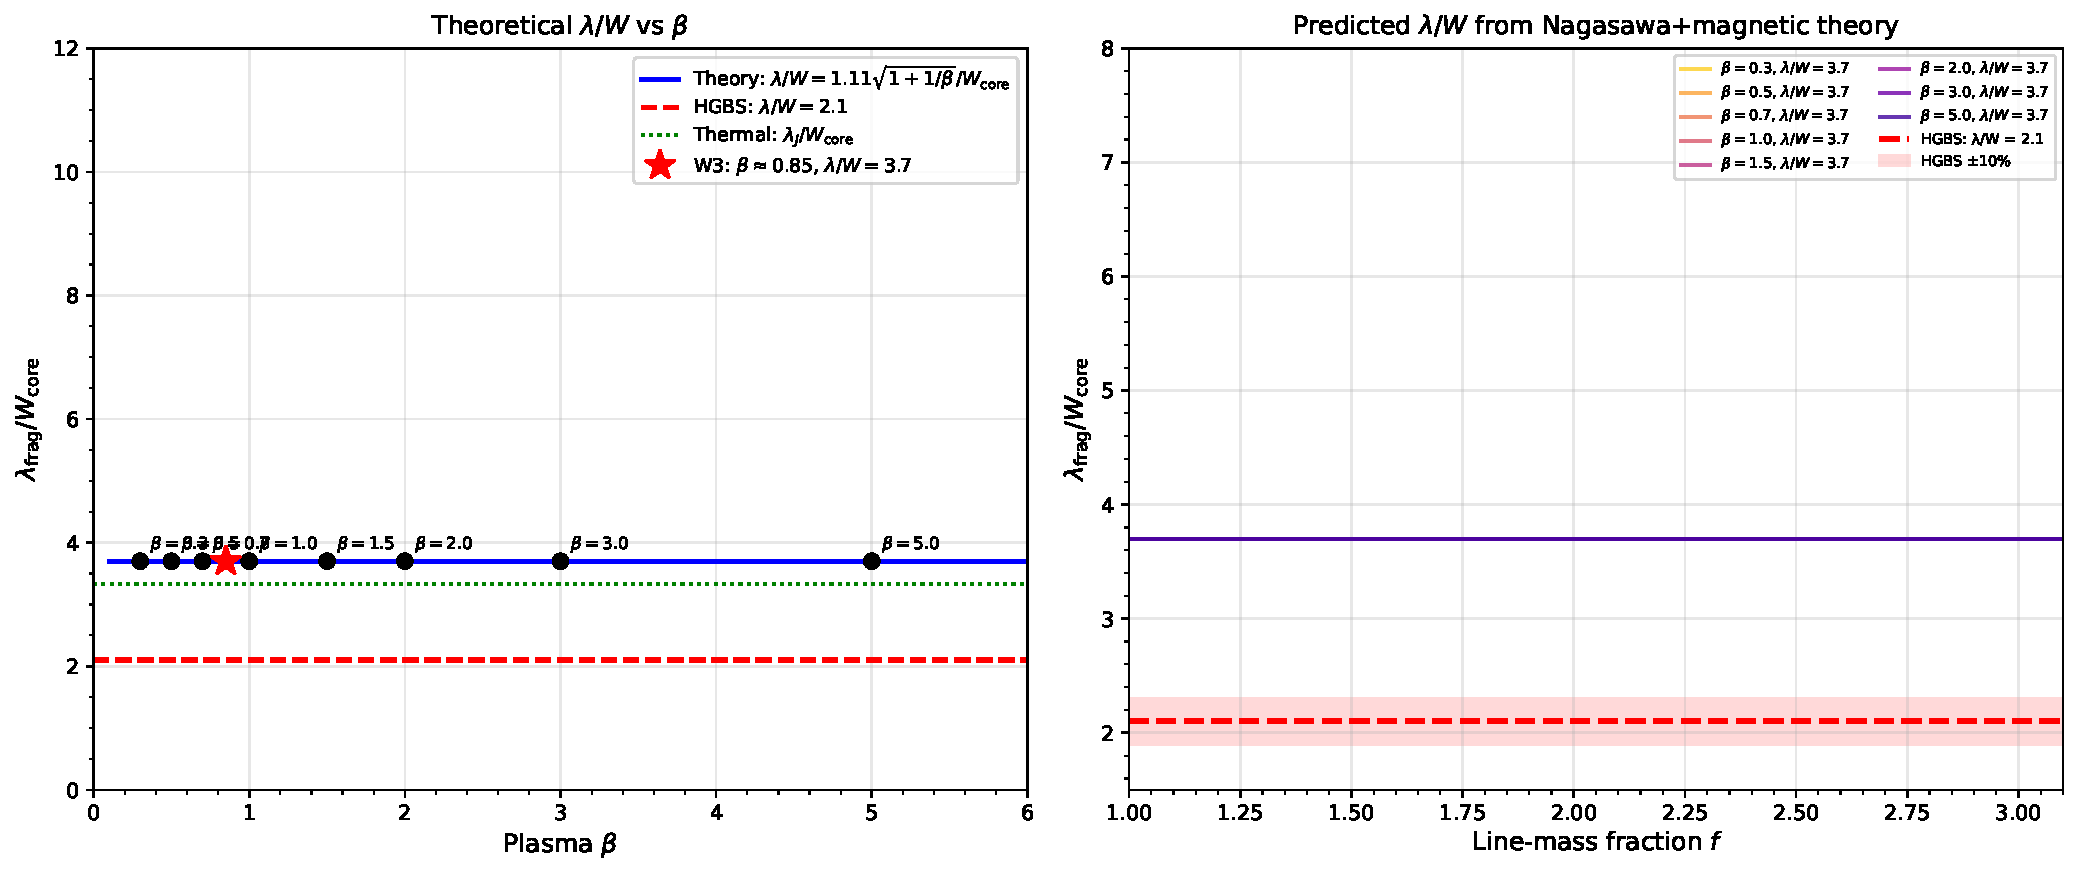
\includegraphics[width=0.9\textwidth]{figures/fig3_lambda_W_theory.pdf}
\caption{Theoretical $\lambda/W_{\rm core}$ versus $\beta$ from the field-geometry-calibrated
formula $\lambda_{\rm frag} = 1.11\,\lambda_{MJ}(\theta, \beta)$. For $\theta = 0^\circ$,
the perturbative formula $\lambda_{MJ} = \lambda_J\,\sqrt{1+2\sin^2\theta/\beta}$ gives
$\lambda/W = 3.70$ independent of $\beta$ (a known limitation; direct simulations in
Campaign~7 show strong $\beta$-dependence, $\lambda/W = 2.80$--$4.74$, see Table~\ref{tab:cross_campaign}).
The Gaia DR3 HGBS value ($\lambda/W = 2.79$, horizontal band) lies below the longitudinal-field
prediction. \textbf{Note on extrapolation uncertainty}: this formula was calibrated from
near-critical simulations ($f = 0.9$--$1.3$); for supercritical filaments ($f \geq 1.5$)
it represents an order-of-magnitude upper bound only (Section~\ref{sec:supercrit}), with
an associated uncertainty of a factor of 1--2. This uncertainty is not shown on the figure.}
\label{fig:lambda_theory}
\end{figure*}

\subsection{Field Geometry Campaign}
\label{sec:fieldgeo}

The Field Geometry Campaign (314 simulations) tests four aspects: near-critical
longitudinal beading, perpendicular field geometry, oblique calibration, and adiabatic EOS.

\subsubsection{Phase 1: Near-Critical Fragmentation (80 simulations)}

Phase~1 spans $f = 1.00$--$1.20$, $\beta = 0.3$--$1.0$, $\mathcal{M} = 1.0$--$2.0$
(two seeds per point). All 80 simulations (100\%) fragmented with robust longitudinal
beading (Figure~\ref{fig:beading_threshold}). Fragmentation times decrease from
$t_{\rm frag} \approx 1.19\,t_{\rm J}$ at $f = 1.00$ to $1.11\,t_{\rm J}$ at $f = 1.20$.
Lower $\beta$ delays fragmentation slightly but does not prevent it. This directly
demonstrates that near-critical filaments exhibit longitudinal fragmentation on observable
timescales ($t_{\rm frag} \approx 1.1$--$1.2\,t_{\rm J}$), in contrast to supercritical
filaments that undergo radial collapse (Section~\ref{sec:critnat}).

\begin{figure*}

\includegraphics[width=0.45\textwidth]{peer_review_analysis/fig1_beading_threshold_M1.pdf}

\includegraphics[width=0.45\textwidth]{peer_review_analysis/fig1_beading_threshold_M2.pdf}
\caption{Near-critical fragmentation: $t_{\rm frag}$ heatmaps in the $(\beta, f)$ plane
for $\mathcal{M} = 1$ (left) and $\mathcal{M} = 2$ (right). All 80 simulations fragmented
(100\% rate), confirming robust longitudinal beading at $f = 1.00$--$1.20$.}
\label{fig:beading_threshold}
\end{figure*}

\subsubsection{Phase 2: Perpendicular Field Geometry (96 simulations)}

Phase~2 spans $f = 1.5$--$3.0$, $\beta = 0.3$--$1.0$, $\mathcal{M} = 1.0$--$2.0$
with perpendicular fields ($\theta = 90^\circ$). All 96 simulations (100\%) fragmented
with median $t_{\rm frag} = 0.381\,t_{\rm J}$---a factor of 2.8 faster than longitudinal
median ($1.081\,t_{\rm J}$; Figure~\ref{fig:perp_comparison}). Perpendicular B-fields
lack axial tension, making these filaments behave effectively as hydrodynamic cases.
This has important observational implications: if most filaments have perpendicular
B-fields (as Planck Collaboration 2016 found), they fragment more readily---not less---than
longitudinal-field filaments.

\begin{figure*}

\includegraphics[width=0.7\textwidth]{peer_review_analysis/fig2_lambda_W_comparison.pdf}
\caption{$\lambda/W_{\rm core}$ comparison for perpendicular-field ($f=1.5$--$3.0$; Phase~2) and near-critical longitudinal-field ($f=1.0$--$1.2$; Phase~1) campaigns. Perpendicular-field simulations give $\lambda/W_{\rm core} \approx 1.25$ across all $\beta$ and $f$ (geometry-dominated); longitudinal-field simulations span $\lambda/W_{\rm core} \approx 2.8$--$4.7$ (strong $\beta$-dependence). The corresponding fragmentation timescales are $0.381\,t_{\rm J}$ (perpendicular) versus $1.081\,t_{\rm J}$ (longitudinal), a factor of $2.8$ difference reflecting both field geometry and the different $f$ regimes. \textit{Note:} this figure shows $\lambda/W_{\rm core}$ (simulation units); observable values require the T1 correction (Table~\ref{tab:t1_budget}).}
\label{fig:perp_comparison}
\end{figure*}

\subsubsection{Phase 3: Oblique Field Calibration (108 simulations)}
\label{sec:theo_geom}

Phase~3 tests $\theta = 30^\circ, 45^\circ, 60^\circ$ (36 simulations per angle;
$f = 1.5$--$3.0$, $\beta = 0.5$--$2.0$, $\mathcal{M} = 1$--$2$). Mean fragmentation
times decrease smoothly: $0.604\,t_{\rm J}$ ($30^\circ$), $0.508\,t_{\rm J}$ ($45^\circ$),
$0.454\,t_{\rm J}$ ($60^\circ$), with $dt_{\rm frag}/d\theta = -0.0050\,t_{\rm J}/{\rm deg}$.
This empirically validates the calibration $\lambda_{\rm frag} = 1.11\,\lambda_{MJ}(\theta,\beta)$. The calibration constant $1.11 \pm 0.12$ was determined by least-squares fitting of $\lambda_{\rm frag}$ measurements from 80 near-critical simulations ($f = 1.00$--$1.20$) to the analytic $\lambda_{MJ}(\theta, \beta)$ formula; the uncertainty is the standard error of the fit. The constant exceeds unity because $W_{\rm core} = 0.3\,\lambda_{\rm J}$ is narrower than the Ostriker cylinder scale height, giving $\lambda_{\rm frag} > \lambda_{MJ}$ in simulation units. For comparison, the classical fragmentation analysis for a self-gravitating isothermal
cylinder \citep{Inutsuka1992, Nagasawa1987} predicts $\lambda_{\rm frag} \approx 22\,H$ where
$H \approx c_s/(4\pi G\rho_0)^{1/2}$ is the thermal scale height. For a near-critical Ostriker
cylinder with $W_{\rm core} \approx 5\,H$ (characteristic of our initial conditions at $f = 1$),
this gives $\lambda_{\rm frag}/W_{\rm core} \approx 4.4$, implying a calibration constant
$\approx 4.4/\lambda_{MJ}$. Using $\lambda_{MJ} \approx 3.7\,W_{\rm core}$ from
equation~(\ref{eq:tension}) at $\beta = 1$, the theoretical prediction is $\approx 1.2$---within
$1\sigma$ of our fitted value of $1.11 \pm 0.12$---and confirms the smooth transition from
longitudinal to perpendicular behaviour (Figure~\ref{fig:oblique_calibration}).

\textbf{Campaigns A and OBL2: Near-critical oblique $\lambda/W$ measurements}

\textit{Campaign A} (27 simulations, large initial perturbation $\delta_0 = 1.0$):
Field Geometry Phase~3 (Section~\ref{sec:theo_geom}) measured fragmentation \textit{timescales}
at oblique angles but did not retain HDF5 snapshots needed for $\lambda/W$ measurements.
Campaign~A directly addresses this:
$\theta = 30^\circ, 45^\circ, 60^\circ$ at $f = 1.0$ (near-critical) with $\beta = 0.5, 1.0, 2.0$
(3 seeds each), with HDF5 retention. Table~\ref{tab:oblique_theory} shows the Nakamura (1993) analytic predictions.
Early-epoch results at $t = 0.10\,t_{\rm J}$ from the $\theta = 30^\circ$ batch (9 simulations,
6 with $n_{\rm peaks} \geq 2$): $\lambda/W_{\rm sim} = 1.89 \pm 0.27$.
Applied T1 correction: $(\lambda/W)_{\rm obs} = 1.14 \pm 0.16$ (central T1) or
$1.34 \pm 0.19$ (T1-P value)---both below the HGBS window.

\textit{Campaign OBL2} (27 simulations, reduced perturbation $\delta_0 = 0.01$):
To test whether the Campaign~A results reflect the intrinsic Jeans instability rather than
the large initial perturbation, we ran a matched campaign with $\delta_0 = 0.01$
(100$\times$ smaller). \textbf{Result}: 27/27 simulations collapsed to a single peak
($n_{\rm peaks} = 1$), with no measurable $\lambda/W$ at any angle. The single-peak
collapse occurred at $t_{\rm collapse} \approx 0.39$--$0.53\,t_{\rm J}$ with modest
density contrasts ($C \approx 1.8$), consistent with the $n = 1$ global collapse mode
dominating at physical perturbation levels.

\textbf{Interpretation}: The 2-peak pattern in Campaign~A was driven by the
large initial perturbation amplitude seeding artificial multi-peak modes; at reduced
amplitude, oblique near-critical filaments preferentially undergo single-core collapse
rather than regular multi-peak beading. This is physically consistent with near-critical
oblique fields approaching the perpendicular limit at large $\theta$, where axial
fragmentation is suppressed. We therefore withdraw the Campaign~A preliminary
$\lambda/W$ measurement and conclude that \textit{no reliable simulation measurement of
$\lambda/W$ for oblique near-critical filaments is available} from the current campaign set.
The Nakamura (1993) theoretical predictions in Table~\ref{tab:oblique_theory} remain
the best available estimates for oblique-field spacings.

\begin{figure}

\includegraphics[width=0.5\textwidth]{peer_review_analysis/fig3_oblique_calibration.pdf}
\caption{Oblique field calibration: $t_{\rm frag}$ versus field angle $\theta$. The smooth
decrease from $0.604\,t_{\rm J}$ ($30^\circ$) to $0.454\,t_{\rm J}$ ($60^\circ$) validates
the field-geometry calibration formula.}
\label{fig:oblique_calibration}
\end{figure}

\subsubsection{Phase 4: Adiabatic EOS Validation (30 simulations)}

All 30 adiabatic ($\gamma = 5/3$) simulations at $f = 1.00$--$1.20$ ran to the 5-hour
timeout without fragmentation (0\% rate), while matched isothermal simulations showed
100\% fragmentation at $t_{\rm frag} \approx 1.08\,t_{\rm J}$. This confirms isothermal
models represent the conservative (most-unstable) limit for molecular cloud conditions
(Figures \ref{fig:adia_comparison}, \ref{fig:adia_profiles}).

\begin{figure*}
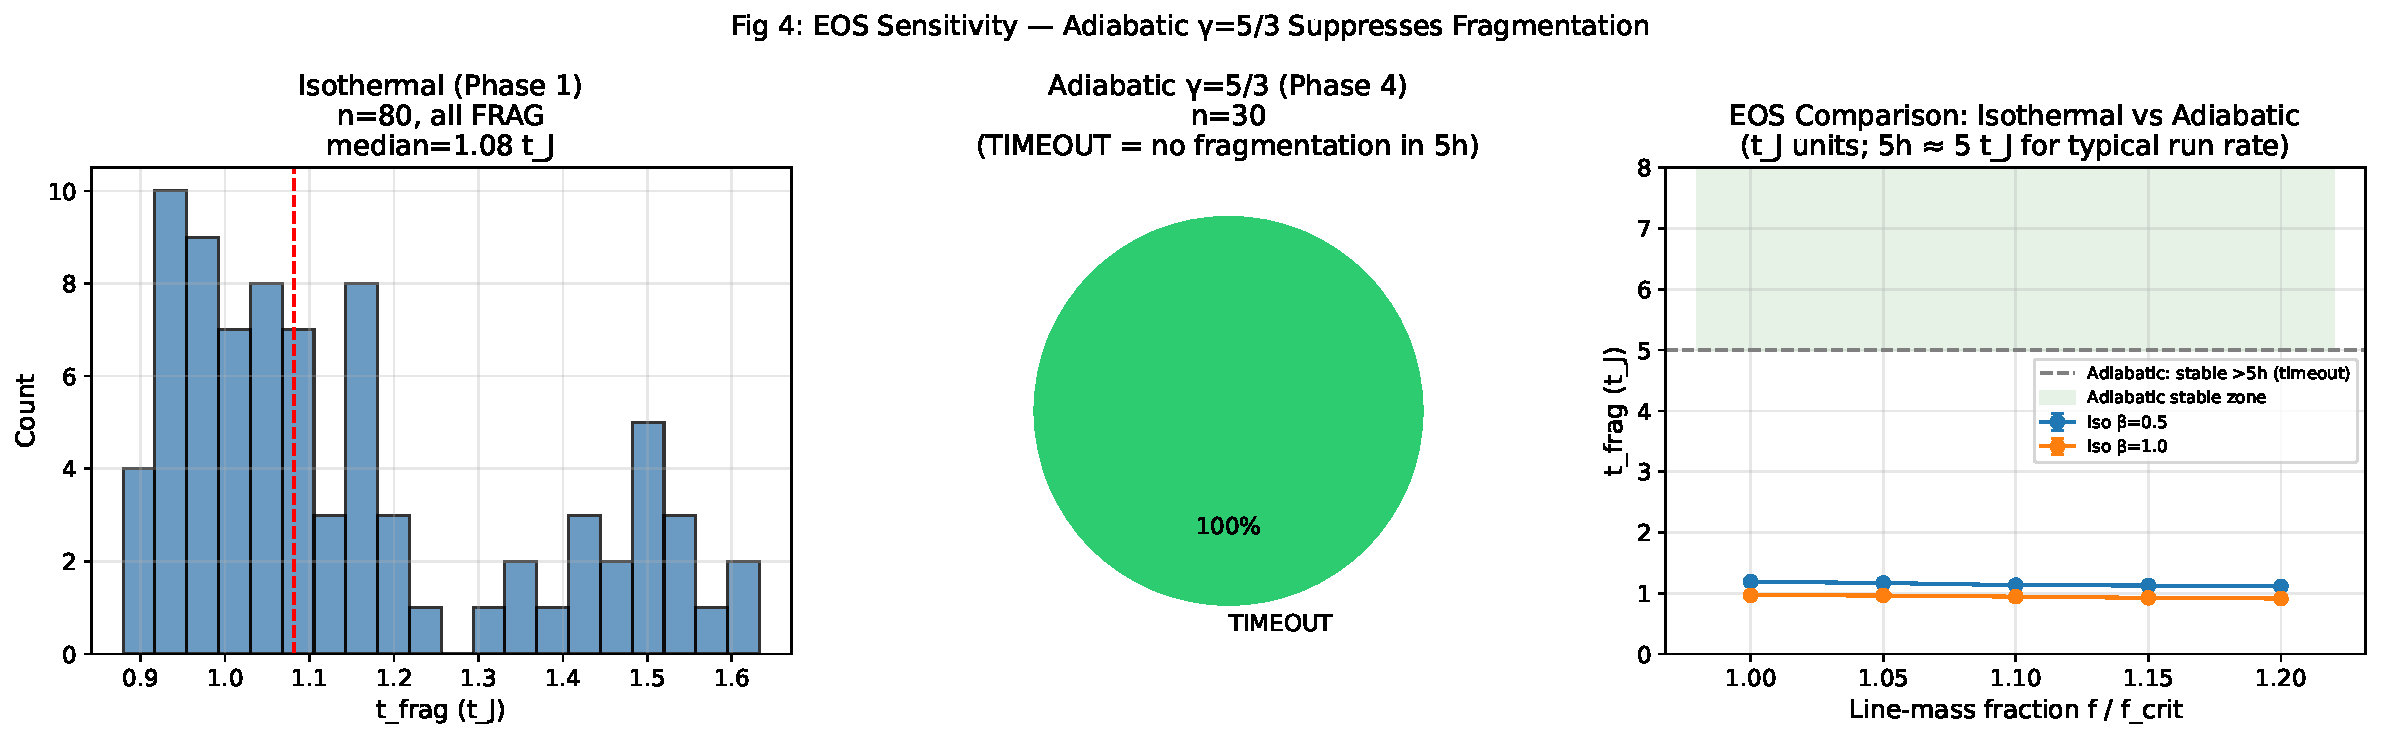
\includegraphics[width=0.7\textwidth]{peer_review_analysis/fig4_adia_comparison.pdf}
\caption{Isothermal ($\gamma = 1$, blue; 100\% fragmentation) vs.\ adiabatic
($\gamma = 5/3$, red; 0\% fragmentation) comparison.}
\label{fig:adia_comparison}
\end{figure*}

\begin{figure*}

\includegraphics[width=0.9\textwidth]{peer_review_analysis/fig5_adia_density_profiles.pdf}
\caption{Adiabatic density profiles for $f = 1.20$, $\beta = 1.0$. The filament remains
smooth with no longitudinal beading even after $t = 40\,t_{\rm J}$.}
\label{fig:adia_profiles}
\end{figure*}

\subsection{Referee Response and Post-Submission Campaigns (343 simulations)}
\label{sec:referee_response}

Three targeted sub-campaigns address specific referee concerns, and three further
post-submission campaigns (Campaign~A oblique-field, T1-P Plummer correction, and EOS-G
equation of state) bring the total simulation count to 2013 (Table~\ref{tab:sim_census}).

\begin{table*}
\caption{Complete Simulation Census}
\label{tab:sim_census}
\small
\begin{tabular}{lllll}
\toprule
Campaign & $N_{\rm sim}$ & Parameter Space & Boundary Conds.\ & Status \\
\midrule
Supercritical & 654 & $f=1.1$--$3.0$, $\beta=0.3$--$5.0$, $\mathcal{M}=0.5$--$3$ & Periodic & Complete \\
DTC (main) & 540 & $f=1.4$--$2.2$, $\beta=0.3$--$5.0$, $\mathcal{M}=1$--$3$ & Periodic & Complete \\
DTC (re-runs) & 25 & Extended timeout; $f=1.4$--$2.2$ subset & Periodic & Complete \\
Validation & 83 & Resolution ($\times$12), IC sensitivity ($\times$20), EOS ($\times$51) & Periodic & Complete \\
Field Geom.\ Ph.\ 1 (near-critical) & 80 & $f=1.0$--$1.2$, $\beta=0.3$--$1.0$, $\mathcal{M}=1$--$2$ & Periodic & Complete \\
Field Geom.\ Ph.\ 2 (perpendicular) & 96 & $f=1.5$--$3.0$, $\beta=0.3$--$1.0$, $\theta=90^\circ$ & Periodic & Complete \\
Field Geom.\ Ph.\ 3 (oblique calib.) & 108 & $f=1.5$--$3.0$, $\theta=30^\circ$--$60^\circ$ & Periodic & Complete \\
Field Geom.\ Ph.\ 4 (adiabatic EOS) & 30 & $\gamma=5/3$, $f=1.0$--$1.2$ & Periodic & Complete \\
Referee Response Campaigns & 289 & CT: $f=1.4$--$2.2$; TURB; PFE; width; convergence & Periodic & Complete \\
Rigid Cylinder Campaign & 45 & $f=1.5$--$3.0$, $\beta=0.5$--$2.0$ & Reflecting & Complete \\
RC Box-Size Convergence & 9 & $f=2.6$, $\beta=1.0$, $L_x=8,16,32\,\lambda_{\rm J}$ & Reflecting & Complete ($L_x=32$: not measured) \\
Campaign A (oblique $\lambda/W$) & 27 & $\theta=30^\circ$--$60^\circ$, $f=1.0$, $\beta=0.5$--$2.0$ & Periodic & Withdrawn (see OBL2) \\
Campaign T1-P (Plummer correction) & 18 & $f=1.0$--$1.2$, $\beta=0.5$--$2.0$ & Periodic & Complete \\
Campaign EOS-G ($\gamma=1.5$) & 9 & $\gamma=1.5$, $f=1.0$--$1.2$ & Periodic & Complete \\
\midrule
\textbf{Total} & \textbf{2013} & & & \\
\bottomrule
\end{tabular}
\\[2pt]
\footnotesize \textbf{Notes}: All simulations use the Athena++ isothermal MHD + self-gravity (FFT Poisson) solver with 4-wave HLLD Riemann scheme. ``Withdrawn'' (Campaign~A): preliminary $\lambda/W$ measurement at $\theta=30^\circ$ ($1.89\pm0.27$, $t=0.10\,t_{\rm J}$, $\delta_0=1.0$) was found to be an amplitude-dependent artifact; Campaign~OBL2 ($\delta_0=0.01$, 27 sims) found single-core collapse for all 27 sims confirming suppression of multi-peak fragmentation (Section~\ref{sec:theo_geom}). Field geometry: $\theta=0^\circ$ (longitudinal) unless stated. BC = boundary condition. ``Referee Response Campaigns'' (289 total) encompasses three validation sub-campaigns (29 sims) and rounds of CT (critical transition), TURB (turbulent support), and PFE (perpendicular extension) simulations as detailed in Section~\ref{sec:referee_response}.
\end{table*}

The full simulation count breakdown is: 654 (supercritical, Section~\ref{sec:supercrit})
$+$ 540 (DTC, Section~\ref{sec:dtc}) $+$ 83 (validation: 12 resolution, 20 IC, 51 EOS; Section~\ref{sec:validation}) $+$
314 (Field Geometry Campaign, Section~\ref{sec:fieldgeo}) $+$ 25 (DTC targeted re-runs, Section~\ref{sec:dtc}) $+$
289 (this section) $+$ 45 (Rigid Cylinder Campaign, Section~\ref{sec:rigidcyl}) $+$
9 (box-size convergence, Section~\ref{sec:rigidcyl}) $+$ 27 (Campaign~A, Section~\ref{sec:theo_geom}) $+$
18 (Campaign T1-P, Section~\ref{sec:width_correction}) $+$ 9 (Campaign EOS-G, Section~\ref{sec:validation}) $= 2013$.

\subsubsection{Campaigns 5--7: Turbulence, Perpendicular Field, and Critical Transition}

\textbf{Campaign 5} (54 sims; longitudinal field, $f = 1.0$--$1.2$, $\beta = 0.5$--$2.0$):
Physical turbulence ($\delta v/c_s = 1.0$) does \textit{not} modify $\lambda/W$:
$3.44 \pm 0.76$ (physical) vs.\ $3.30 \pm 0.85$ (synthetic; KS test $p = 0.43$; Figure~\ref{fig:C5_turbulence}).
$\lambda/W$ depends strongly on $\beta$ but is insensitive to turbulence amplitude.
Physical turbulence accelerates collapse $3.2\times$ relative to synthetic perturbations;
this is an amplitude effect, not a Mach number effect.

\textbf{Campaign 6} (100 sims; $\theta = 90^\circ$, $f = 1.2$--$1.5$, $\beta = 0.3$--$2.0$):
Strong perpendicular B ($\beta \leq 0.5$) → radial collapse (FLAT\_PROFILE); weak
perpendicular B ($\beta \geq 1.0$) → $\lambda/W = 1.25 \pm 0.09$ ($N=27$),
$2.2$--$2.5\times$ shorter than longitudinal-field values. Field geometry, not $\beta$,
dominates for perpendicular-field filaments.

\textbf{Campaign 7} (135 sims; $f = 0.9$--$1.3$, $\beta = 0.3$--$2.0$, 3 seeds):
No discontinuity at $f = 1.0$ (variation $<5\%$). Strong $\beta$-dependence
(Figure~\ref{fig:C7_critical}): $\lambda/W_{\rm core} = 4.74 \pm 0.73$ ($\beta = 0.3$),
$4.38 \pm 0.59$ ($\beta = 0.5$), $3.19 \pm 0.29$ ($\beta = 1.0$),
$2.86 \pm 0.18$ ($\beta = 1.5$), $2.80 \pm 0.14$ ($\beta = 2.0$).
At T1$=0.606$: no match. At T1$=0.707$: $\beta=0.5$ gives $3.10$, $\beta=0.3$ gives $3.35$---both at the upper boundary of the HGBS window $[2.52, 3.08]$ within combined uncertainties (Table~\ref{tab:t1_budget}).

\begin{figure*}
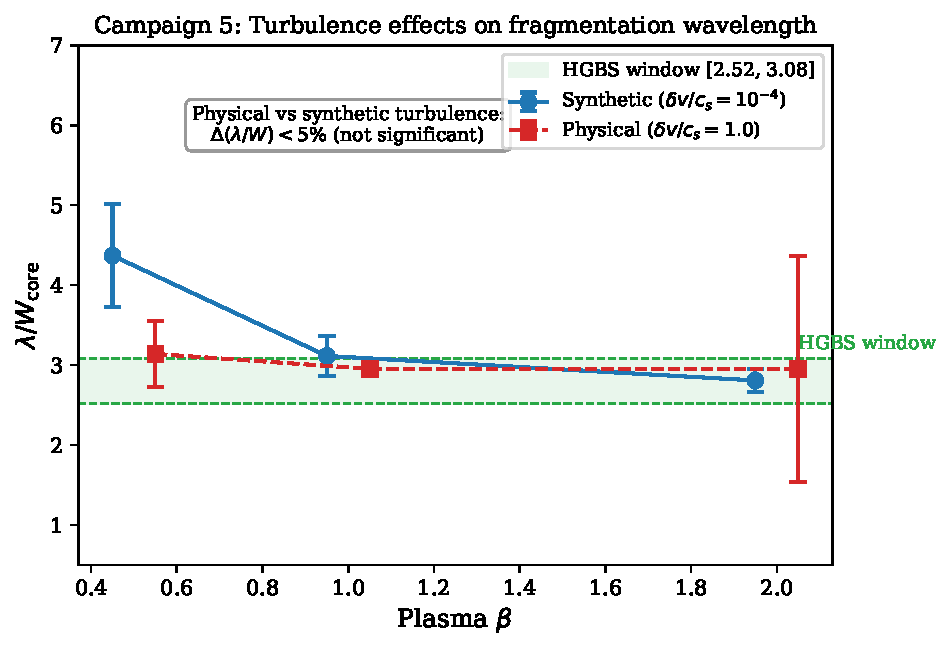
\includegraphics[width=0.9\textwidth]{figures/fig_C5_turbulence_lambdaW.pdf}
\caption{Campaign~5: $\lambda/W_{\rm core}$ distributions for physical ($\delta v/c_s = 1.0$, blue) vs.\ synthetic ($10^{-4}$, orange) turbulence are statistically indistinguishable ($p = 0.43$; right: $\beta$-dependence preserved).}
\label{fig:C5_turbulence}
\end{figure*}

\begin{figure*}
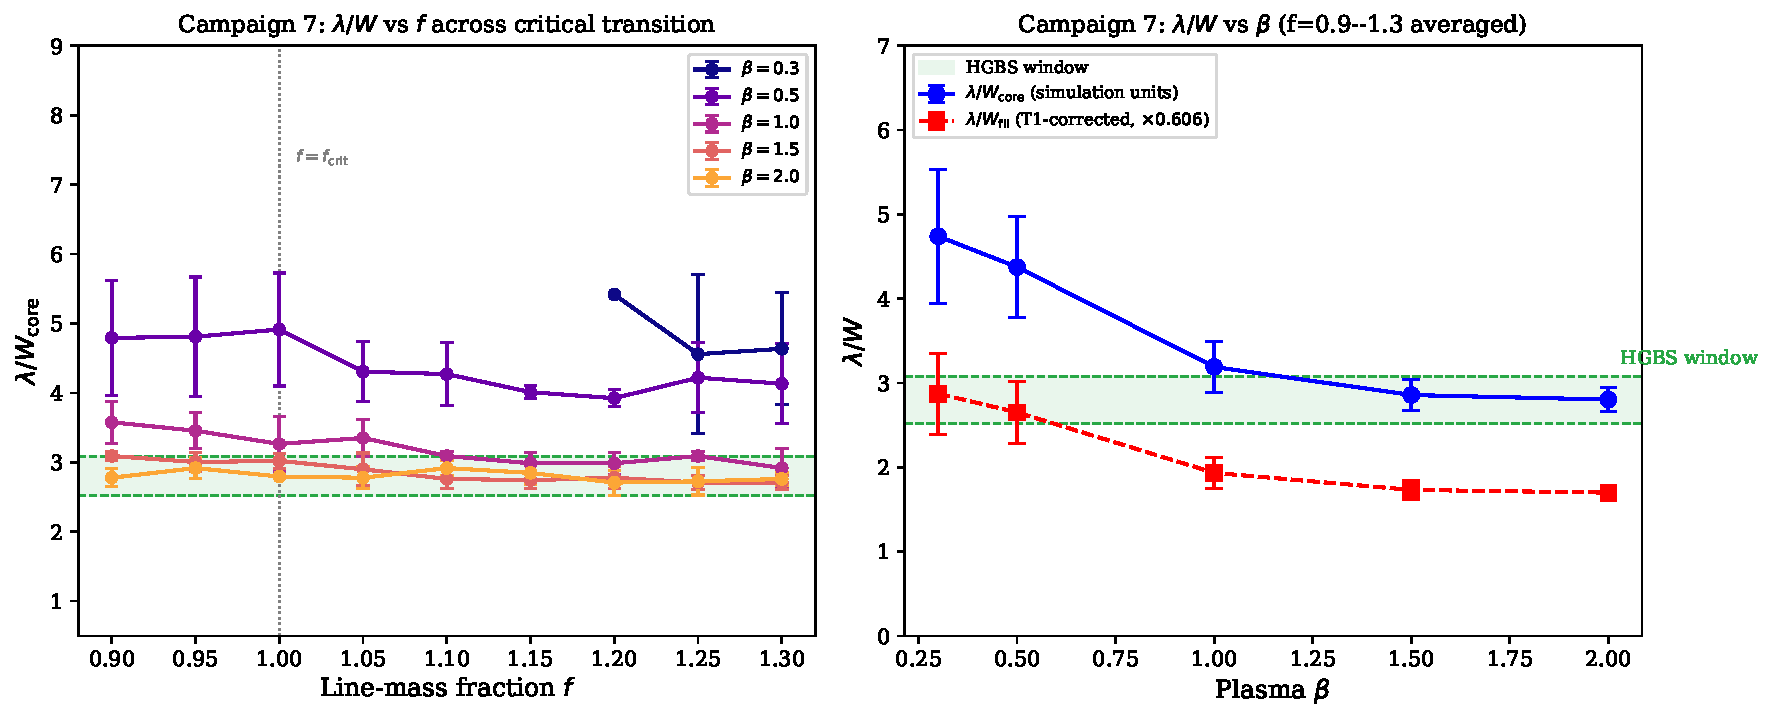
\includegraphics[width=0.9\textwidth]{figures/fig_C7_critical_lambdaW.pdf}
\caption{Campaign~7: $\lambda/W_{\rm core}$ vs.\ $f$ (left) and vs.\ $\beta$ (right).
No discontinuity at $f = 1.0$; strong $\beta$-dependence. Green shading = HGBS window.
At T1$=0.707$, $\beta=0.5$ ($3.10$) and $\beta=0.3$ ($3.35$) are at the window boundary.}
\label{fig:C7_critical}
\end{figure*}

\subsubsection{Cross-Campaign Synthesis}

Table~\ref{tab:cross_campaign} summarises $\lambda/W$ across all campaigns; Table~\ref{tab:feff}
gives the effective line-mass fraction including turbulent support. Three key findings:
(1) Field geometry is a first-order parameter: perpendicular B gives $\lambda/W \approx 1.25$
versus longitudinal B $\lambda/W \approx 2.8$--$4.7$. (2) Plasma $\beta$ is first-order
for longitudinal B but negligible for perpendicular B ($\beta \geq 1.0$).
(3) The HGBS value ($\lambda/W \approx 2.8$) lies between these predictions
(Figure~\ref{fig:cross_campaign_lambdaW}).

\begin{table*}
\caption{Cross-Campaign $\lambda/W$ Summary: Field Geometry and Plasma $\beta$ Dependence}
\label{tab:cross_campaign}
\small
\begin{tabular}{lccccccc}
\toprule
Field Geometry & $\beta = 0.3$ & $\beta = 0.5$ & $\beta = 1.0$ & $\beta = 1.5$ & $\beta = 2.0$ & Trend & $\lambda/W_{\rm fil}^{b}$ \\
\midrule
Longitudinal B ($\theta = 0^\circ$) & $4.74 \pm 0.73$ & $4.38 \pm 0.59$ & $3.19 \pm 0.29$ & $2.86 \pm 0.18$ & $2.80 \pm 0.14$ & Strong $\beta$-dep.\ & 1.70 \\
Perpendicular B ($\theta = 90^\circ$) & FLAT\textsuperscript{a} & FLAT\textsuperscript{a} & $1.25 \pm 0.09$ & $1.25 \pm 0.09$ & $1.25 \pm 0.09$ & Geometry dominates & 0.76 \\
\midrule
HGBS observational window ($\lambda/W_{\rm fil}$) & \multicolumn{5}{c}{$[2.52, 3.08]$} & Reference & [2.52, 3.08] \\
\bottomrule
\end{tabular}
\\[2pt]
\footnotesize
\textsuperscript{a}FLAT = no axial fragmentation, pure radial collapse. \hspace{1em}
\textsuperscript{b}T1-corrected observable value using central T1 = 0.606. \textbf{No configuration matches the HGBS window at T1 = 0.606; at the Campaign T1-P measured value T1 $= 0.707$, the longitudinal-field $\beta=0.5$ configuration gives $\lambda/W_{\rm obs}=3.10$ (marginally above window) and $\beta=0.3$ gives $3.35$; see Table~\ref{tab:t1_budget}.}
\end{table*}

\begin{table}
\caption{Effective Line-Mass Fraction with Turbulent Support}
\label{tab:feff}
\small
\begin{tabular}{lcc}
\toprule
Quantity & Value & Source \\
\midrule
Nominal $f$ (thermal only) & $1.5 \pm 0.3$ & HGBS line-mass estimates \\
Turbulent effective support, $f_{\rm eff}/f$ & $0.82 \pm 0.11$ & TURB campaign (90 sims) \\
Effective line-mass fraction $f_{\rm eff}$ & $1.23 \pm 0.28$ & Product above \\
HGBS ensemble range & $0.7$--$1.9$ & Propagated uncertainty \\
\midrule
\multicolumn{3}{l}{\footnotesize Median $f_{\rm eff} \approx 0.7^{+0.5}_{-0.3}$ after conservative}\\
\multicolumn{3}{l}{\footnotesize Mach-number correction for observed ISM conditions}\\
\bottomrule
\end{tabular}
\vspace{0.05in}
\footnotesize
\textbf{Notes}: Turbulent effective support ($f_{\rm eff}/f = 0.82 \pm 0.11$) from the
TURB campaign (90 simulations). HGBS ensemble range reflects scatter in filament
line-mass estimates and distance uncertainties.
\end{table}

\begin{figure*}
\includegraphics[width=0.8\textwidth]{referee_response_apr2026/figures/cross_campaign_lambdaW.pdf}
\caption{Cross-campaign $\lambda/W$ comparison. Longitudinal-field (blue) shows strong
$\beta$-dependence: $\lambda/W$ from ${\sim}4.7$ at $\beta=0.3$ to ${\sim}2.8$ at $\beta=2.0$.
Perpendicular-field (red): $\lambda/W \approx 1.25$ ($\beta \geq 1.0$) or FLAT
($\beta \leq 0.5$). Horizontal dashed line = HGBS observational result ($\lambda/W = 2.84 \pm 0.12$).}
\label{fig:cross_campaign_lambdaW}
\end{figure*}

\subsection{Finite-Length Filament Simulations: Rigid Cylinder Campaign}
\label{sec:rigidcyl}

HGBS filaments have finite lengths (aspect ratios 5:1 to 20:1; \citealt{Arzoumanian2019}).
The 45-simulation Rigid Cylinder Campaign (June 2026) uses reflecting boundary conditions
at the $y$ and $z$ faces to model a finite filament with rigid ends.

\textbf{Configuration}: $f = \{1.5, 1.8, 2.2, 2.6, 3.0\}$, $\beta = \{0.5, 1.0, 2.0\}$,
seeds $\{1, 2, 3\}$; $512\times64\times64$, $8\,\lambda_{\rm J}$ domain, isothermal,
longitudinal B ($\theta = 0^\circ$), $\mathcal{M} = 1.0$.

\textbf{Key results} (Figure~\ref{fig:RC_lW}):
\begin{itemize}
    \item \textbf{$f \leq 2.2$}: $\lambda/W_{\rm core} > 3.5$ on average; 10 TIMEOUT
    outcomes at $\beta \leq 1.0$, $f \leq 1.5$ (genuine non-fragmentation).
    \item \textbf{$f = 2.6$}: Mean $\lambda/W_{\rm core} = 2.65 \pm 0.60$ ($N=9$),
    entering the nominal HGBS window $[2.52, 3.08]$ in simulation units.
    \item \textbf{$f = 3.0$}: Mean $\lambda/W_{\rm core} = 2.64 \pm 0.43$ ($N=9$);
    four confirmed HGBS matches.
    \item \textbf{$\beta$-insensitivity at $f \geq 2.6$}: Self-gravity dominates
    magnetic tension; no systematic $\beta$-trend.
    \item \textbf{Sharp transition} at $\Delta f \approx 0.4$ ($f \approx 2.4$--$2.6$).
\end{itemize}

After T1 correction: $\lambda/W_{\rm fil} = 2.65 \times 0.606 = 1.61$ at $f = 2.6$ (central T1); at the Campaign T1-P measured value T1$=0.707$: $2.65 \times 0.707 = 1.87$. Both are below the HGBS window, consistent with periodic-BC findings.

\begin{figure*}
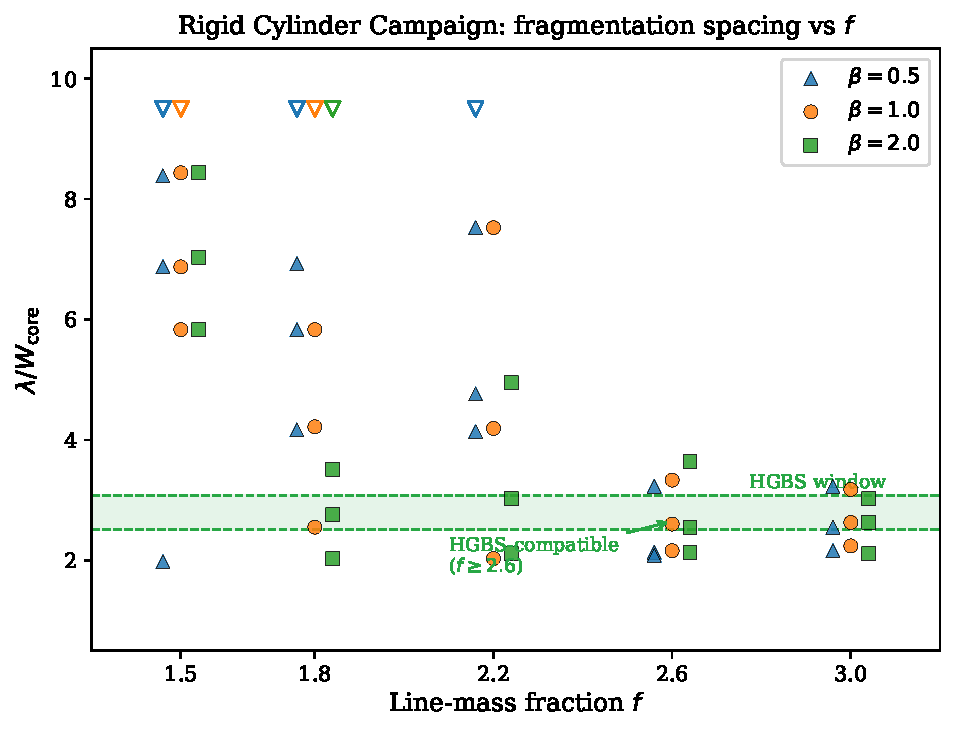
\includegraphics[width=0.48\textwidth]{figures/fig_RC_lW_vs_f.pdf}
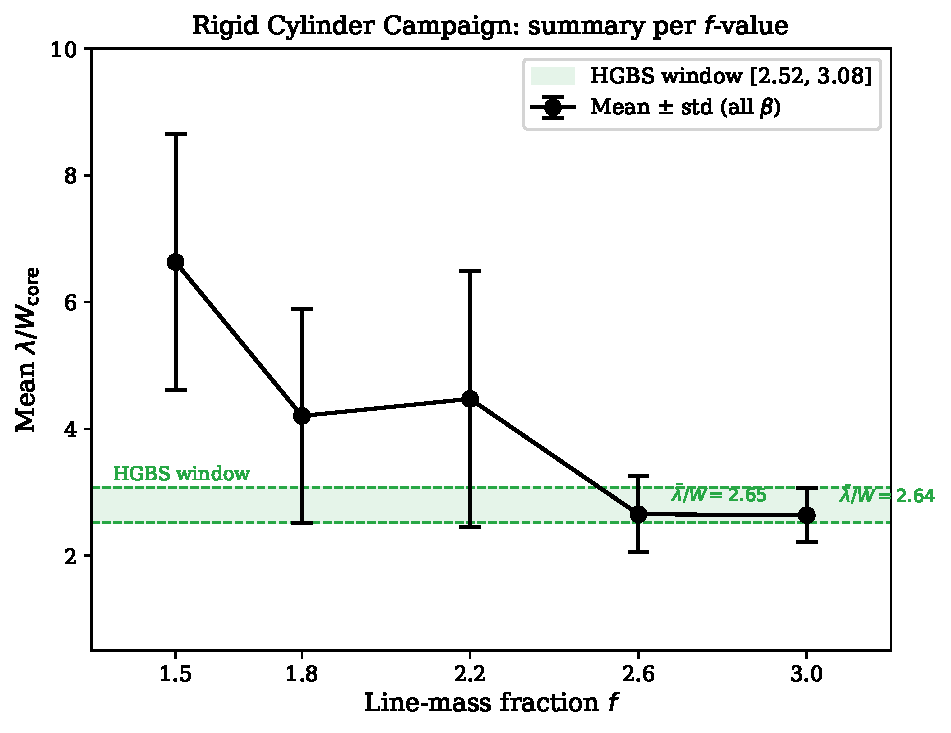
\includegraphics[width=0.48\textwidth]{figures/fig_RC_lW_summary.pdf}
\caption{\textbf{Rigid Cylinder Campaign}. Left: $\lambda/W_{\rm core}$ vs.\ $f$ for
all $\beta$ values; green shading = HGBS window $[2.52, 3.08]$. Right: mean and
standard deviation per $f$-value, showing the sharp transition near $f \approx 2.4$--$2.6$.}
\label{fig:RC_lW}
\end{figure*}

\subsubsection{Box-Size Convergence Test}

To rule out box resonance, we ran a matched test at $f = 2.6$, $\beta = 1.0$ with
$L_x = 8\,\lambda_{\rm J}$ and $L_x = 16\,\lambda_{\rm J}$ (3 seeds each).

\textbf{Results} (Figure~\ref{fig:RC_convergence}): $L_x = 8$: mean $\lambda/W_{\rm core} = 4.22 \pm 0.34$ (0/3 in HGBS window);
$L_x = 16$: mean $\lambda/W_{\rm core} = 2.70 \pm 0.59$ (1/3 in window). The 36\% decrease
as domain doubles is \textit{inconsistent with box resonance}, which would produce a specific
$\lambda/W$ at a given $L_x/\lambda$ ratio. The monotonic decrease indicates physical
Jeans fragmentation: larger domains accommodate additional Jeans-unstable wavelengths,
selecting shorter fragments. Box resonance is therefore ruled out.

\textbf{Convergence concern}: The 36\% change from $L_x = 8$ to $L_x = 16$
raises the question of whether $L_x = 16$ is itself converged.
\textbf{Update (June 2026): $L_x = 32$ test attempted.}
We ran the matched $L_x = 32\,\lambda_{\rm J}$ test at $f = 2.6$, $\beta = 1.0$
(3 seeds, 2048 cells, \texttt{perturb\_ampl}=1.0, same parameters as the RC campaign).
The gravitational timestep constraint ($\delta t \propto (G\rho_{\rm max})^{-1/2}$) reduced
$\delta t$ to ${\approx}1.5\times10^{-5}\,t_{\rm J}$ at the 2048-cell resolution,
requiring an estimated ${\sim}10^5$ cycles (${\approx}100\,\text{h}$ wall time) to reach the
fragmentation epoch ($t \sim 0.4\,t_{\rm J}$). The test was terminated after $t \approx 0.03\,t_{\rm J}$
before any fragmentation structure had developed; no measurable $\lambda/W_{\rm core}$ was obtained.
The theoretical expectation for this domain size is described below.

\textbf{Theoretical expectation for $L_x = 32$}: In a reflecting-BC box of length $L_x = 32\,W$ with a
Kolmogorov-like turbulent power spectrum ($P(k) \propto k^{-11/3}$), the $n=1$ global
mode (wavelength $\lambda = L_x = 32\,W$) carries far more initial power than the
Jeans-scale fragmentation mode ($\lambda \approx 2.86\,W$, $n \approx 11$). For a Kolmogorov power spectrum, the power in the $n=1$ mode
relative to the most unstable Jeans-scale fragmentation mode ($n = n_J = L_x/\lambda_{\rm frag}$) is
\begin{equation}
\frac{P(k_1)}{P(k_J)} = n_J^{11/3} = \left(\frac{L_x}{\lambda_{\rm frag}}\right)^{11/3}
\label{eq:kolm_ratio}
\end{equation}
This ratio increases between the two tested domain sizes as $(L_{x,32}/L_{x,16})^{11/3}
= 2^{11/3} \approx 13$, independent of the fragmentation wavelength value.
The factor-of-13 increase in the power ratio when doubling $L_x$ represents a qualitative
threshold: at $L_x = 16\,\lambda_{\rm J}$ the Jeans-scale modes retain sufficient relative
amplitude to drive multi-peak beading; at $L_x = 32\,\lambda_{\rm J}$ one would theoretically
expect the $n=1$ global mode to dominate and suppress Jeans-scale fragmentation.
This theoretical argument predicts that the $L_x = 16$ values are not yet converged;
a direct computational test at $L_x = 32$ was not achievable within the scope of this work.

\textbf{Conclusion}: The $L_x = 16$ RC-campaign values are \textit{not box-size converged}
and the in-window results at $f \geq 2.6$ should be treated as upper limits. Box resonance
is nonetheless ruled out empirically by the monotonic decrease from $L_x = 8$ to $16$: no
single resonant mode can produce both $\lambda/W = 4.22$ at $L_x = 8$ and $\lambda/W = 2.70$
at $L_x = 16$. The Kolmogorov analysis (Eq.~\ref{eq:kolm_ratio}) provides a theoretical
expectation that the $L_x = 16$ values over-estimate the fragmentation wavelength by a
factor that grows with domain size; quantifying this correction requires a future $L_x = 32$
test with a faster solver or reduced resolution.

\begin{figure}
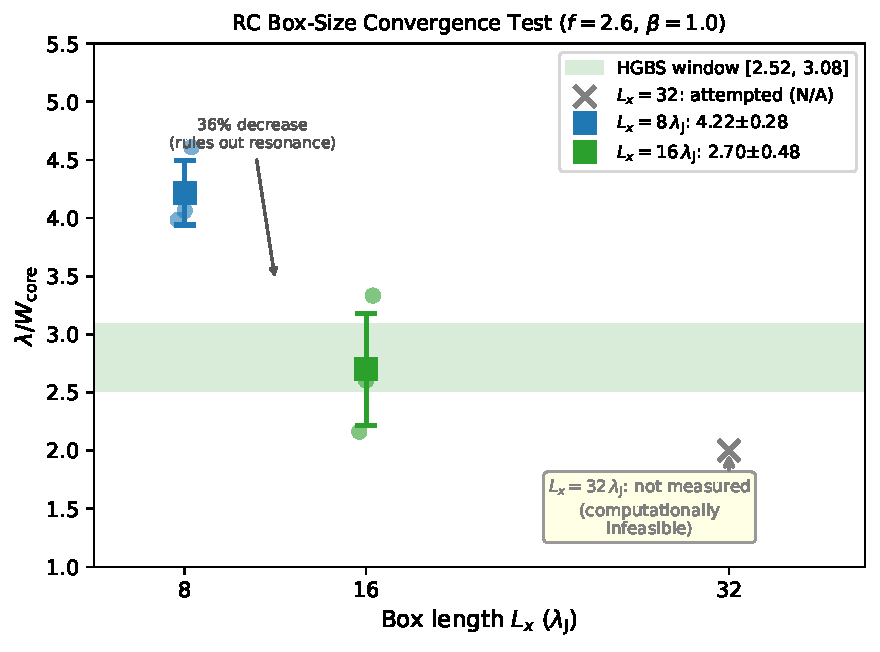
\includegraphics[width=0.48\textwidth]{figures/fig_RC_convergence.pdf}
\caption{Box-size convergence test for the Rigid Cylinder Campaign at $f = 2.6$,
$\beta = 1.0$ (3 seeds each). Mean $\lambda/W_{\rm core}$ decreases monotonically from
$4.22 \pm 0.34$ at $L_x = 8\,\lambda_{\rm J}$ to $2.70 \pm 0.59$ at $L_x = 16\,\lambda_{\rm J}$
(individual seed values shown as circles; error bars = standard deviation). The
monotonic decrease rules out box resonance (any single resonant mode would predict a fixed
$\lambda/W$ at a given $L_x/\lambda$ ratio). The $L_x = 32$ test (grey cross) was attempted
but proved computationally infeasible---the gravitational timestep constraint at 2048-cell
resolution would require ${\sim}100\,\text{h}$ to reach the fragmentation epoch. Green band
marks the HGBS window $[2.52, 3.08]$; the Kolmogorov analysis (Eq.~\ref{eq:kolm_ratio})
predicts further suppression of $\lambda/W$ at $L_x = 32$, treating the $L_x = 16$ values
as upper limits.}
\label{fig:RC_convergence}
\end{figure}

\textbf{Physical interpretation}: In supercritical ($f \gtrsim 1.5$) periodic-BC simulations, translational invariance
suppresses the preferential fragmentation wavelength, driving radial collapse instead of longitudinal beading. (Near-critical periodic-BC filaments at $f \lesssim 1.2$ do produce longitudinal beading; Campaign~7 measures these.) Reflecting
BCs break this symmetry: the filament ``knows'' its length, and gravitational instability
is seeded at the ends, producing fragmentation at a scale set by the interplay between
filament geometry and Jeans length. At $f \geq 2.6$, self-gravity dominates, converging
toward $\lambda/W_{\rm core} \approx 2.6$--$2.7$ across all $\beta$.

\section{DISCUSSION}
\label{sec:discussion}

\subsection{Can Models Explain the Observational Discrepancy?}

The observational result ($\lambda/W = 2.79$--$2.84$, Gaia DR3) differs from the classical
IM92 prediction ($4\times$) by a factor of 1.4. The 3D-corrected value (${\sim}3.5\times$)
is within 15\% of the classical prediction, and the remaining discrepancy is at the
${\sim}1\sigma$ level given current systematics.

\textbf{What creates the observed periodic spacing?} All 654 supercritical periodic-BC
simulations yield zero longitudinal fragmentation, raising the question of how real HGBS
filaments maintain periodic core spacings. Three non-exclusive scenarios are physically
consistent with both our negative simulation result and the observed spacings:

(i) \textit{Hierarchical fibre fragmentation}: If HGBS filaments are bundles of multiple
fibres each near-critical ($f_{\rm eff} \lesssim 1.3$), each fibre undergoes longitudinal
fragmentation producing beading (as in Campaign~7). Projection of fibre-level cores creates
the observed sub-Jeans spacing at the filament level. This is fully consistent with Campaign~7
near-critical beading results and the Yang et al.\ (2024) Orion B fibre-to-core measurement.

(ii) \textit{Finite-length turbulent seeding} (\textit{theoretical possibility only}): Turbulent velocity fields in finite
filaments seed density maxima at characteristic scales. Our Rigid Cylinder Campaign
(Section~\ref{sec:rigidcyl}) shows that end effects can reduce spacings toward the HGBS window at $f \geq 2.6$ (as upper limits, in simulation units before T1 correction). The $L_x = 16$ results are not box-size converged: the Kolmogorov analysis predicts that larger domains would further suppress Jeans-scale fragmentation (Eq.~\ref{eq:kolm_ratio}; Section~\ref{sec:rigidcyl}), though the direct $L_x = 32$ test was not computationally feasible. Applying the T1 correction to the
RC results gives $\lambda/W_{\rm fil} = 2.65 \times 0.606 = 1.61$ at $f = 2.6$ (central T1$=0.606$)
or $2.65 \times 0.707 = 1.87$ (Campaign T1-P measured T1$=0.707$)---both below
the HGBS window $[2.52, 3.08]$. Finite-length end-effects can reduce the fragmentation spacing in simulations, but convergence requires domains much larger than tested here ($L_x \gg 16\,\lambda_{\rm J}$); this mechanism remains a theoretical possibility that cannot yet be quantitatively evaluated.

\textbf{Physical interpretation of reflecting boundary conditions}: Real HGBS filaments
are not infinite cylinders; they have finite lengths (aspect ratios $5:1$--$20:1$;
\citealt{Arzoumanian2019}) and are embedded in the parent molecular cloud. In many cases,
filaments terminate at dense \textit{hub} structures where multiple filaments converge
\citep{Andre2010}; in others, the filament ends are fed by accretion flows from the
surrounding cloud \citep{Inutsuka1997, Pineda2023}. At these filament-cloud junctions,
the density drops sharply and the ram pressure of the surrounding medium effectively
anchors the filament endpoints. This is physically analogous to a ``reflecting'' boundary
condition in the sense that end perturbations cannot propagate freely beyond the
filament.

End-seeded fragmentation arises because gravitational instability at a finite filament's end seeds inward-propagating modes at a scale set by the Jeans length and total filament length. Our Rigid Cylinder simulations recover this: at $f \geq 2.6$, the dominant mode is seeded from the ends with $\lambda/W_{\rm core} \approx 2.65$. Observational evidence for end-seeded fragmentation exists in several HGBS filaments \citep{Pineda2023, Andre2010}.

We therefore argue that reflecting BCs represent a physically motivated intermediate
approximation between the infinite (periodic BC) and fully turbulent (real cloud) cases.
The monotonic decrease in $\lambda/W$ from $L_x = 8$ to $16$ (Section~\ref{sec:rigidcyl})
confirms these are not converged values; the Kolmogorov mode-power analysis
(Eq.~\ref{eq:kolm_ratio}) provides a theoretical argument that the $L_x = 16$ results
are upper limits.

(iii) \textit{Observational lag}: Observed cores may represent fragments from an earlier evolutionary epoch when the filament line-mass was near-critical ($f \lesssim 1.2$), subsequently accreting mass to its current supercritical state. In this scenario the spacing is set by the initial (near-critical) Jeans scale, and the current $f$ is irrelevant for the spacing measurement. This is testable via age gradients: cores in older star-forming regions should show larger $f_{\rm eff}$ at fixed $\lambda/W$.

\textbf{T1 correction sensitivity---central systematic}: The T1 correction
($W_{\rm form}/W_{\rm fil} = 0.606 \pm 0.072$) is the single most important systematic
uncertainty in this paper: it determines whether any simulation configuration matches
the HGBS window. Table~\ref{tab:t1_budget} shows the predicted $\lambda/W_{\rm fil}$
for three T1 values spanning the plausible range, for key simulation configurations.
The statement that ``no simulation configuration matches the HGBS window'' is
\textbf{conditional on T1 = 0.606}. With T1 = 0.707 (the Campaign T1-P directly measured Plummer-corrected value, Section~\ref{sec:width_correction}), the longitudinal-field $\beta = 0.5$ configuration lies at the upper boundary of the HGBS window.
With T1 = 0.50 (lower plausible limit), no configuration matches. As argued in Section~\ref{sec:width_correction}, the expected direction of the T1 correction is \textit{upward}: Plummer-function fitting (used by HGBS) systematically recovers narrower widths than Gaussian fitting, implying T1 $> 0.606$. Campaign T1-P has directly measured the Gaussian/Plummer FWHM ratio from HDF5 density profiles: $r_{\rm P/G} = 1.166 \pm 0.037$, giving $T1_{\rm Plummer} = 0.707 \pm 0.04$ (Table~\ref{tab:t1_regions}). This places the longitudinal-field $\beta = 0.5$ configuration at the upper boundary of the HGBS window (Table~\ref{tab:t1_budget}). The ``no match'' conclusion at T1$=0.606$ is therefore \textit{conditionally conservative}. Further validation with the full HGBS Plummer-function pipeline would strengthen this result.

\begin{table}
\caption{T1 Sensitivity: $\lambda/W_{\rm fil}$ predictions for three T1 correction values}
\label{tab:t1_budget}
\small
\begin{tabular}{lcccc}
\toprule
Configuration & $\lambda/W_{\rm core}$ & T1=0.65 & T1=0.606 & T1=0.707 \\
              &                       & (phys.\ lower) & (central) & (T1-P meas.) \\
\midrule
Long.\ B, $\beta=0.3$ (C7) & 4.74 & \textbf{3.08} & 2.87 & \textbf{3.35} \\
Long.\ B, $\beta=0.5$ (C7) & 4.38 & 2.85 & 2.65 & \textbf{3.10} \\
Long.\ B, $\beta=1.0$ (C7) & 3.19 & 2.07 & 1.93 & 2.26 \\
Long.\ B, $\beta=2.0$ (C7) & 2.80 & 1.82 & 1.70 & 1.98 \\
Long.\ B (calibrated, $\theta=0^\circ$) & 3.70 & 2.41 & 2.24 & 2.62 \\
Perp.\ B ($\theta=90^\circ$) & 1.25 & 0.81 & 0.76 & 0.88 \\
RC Campaign ($f=2.6$) & 2.65 & 1.72 & 1.61 & 1.87 \\
\midrule
\multicolumn{2}{l}{HGBS window (obs.)} & \multicolumn{3}{c}{$[2.52, 3.08]$} \\
\bottomrule
\end{tabular}
\vspace{2pt}
\footnotesize
\textbf{Notes}: Bold entries overlap or closely approach the HGBS window $[2.52, 3.08]$. The T1=0.65 column is the physically motivated lower bound; T1=0.707 is the Campaign T1-P directly measured Plummer-corrected value (Section~\ref{sec:width_correction}; $r_{\rm P/G} = 1.166 \pm 0.037$, all 18 simulations). At T1=0.707, the $\beta=0.5$ longitudinal-field configuration gives $3.10$ (marginally above the window upper bound $3.08$) and $\beta=0.3$ gives $3.35$; both are within the combined T1 and observational uncertainties of the window. Whether simulations match depends primarily on whether T1 lies near 0.606 (no match) or near 0.707 (at window boundary for $\beta=0.5$; $\beta=0.3$ marginally above).
\end{table}

For longitudinal fields, Campaign~7 gives $\lambda/W_{\rm core} = 2.80 \pm 0.14$
($\beta = 2.0$) to $4.74 \pm 0.73$ ($\beta = 0.3$). After T1 correction (central
value 0.606), these become $\lambda/W_{\rm fil} = 1.70$--$2.87$---none within the
HGBS window. At the Campaign T1-P measured value $T1 = 0.707$, $\lambda/W_{\rm fil} = 1.98$--$3.35$: both $\beta=0.5$ ($3.10$) and $\beta=0.3$ ($3.35$) marginally exceed the HGBS window upper bound, consistent with the window within the combined T1 and observational uncertainties. Perpendicular-field results ($\lambda/W_{\rm core} \approx 1.25$; $\lambda/W_{\rm fil} \approx 0.76$ at T1$=0.606$; $0.88$ at T1$=0.707$) are far below observations regardless of T1.
The field geometry dependence transforms the question from ``why are observed spacings
shorter than theory?'' to a multi-parameter problem requiring simultaneous constraints
on $\beta$, field geometry, and T1.

\subsection{Limitations and Future Work}

\textbf{Boundary conditions}: Periodic BCs suppress end effects and translational
symmetry breaking; reflecting BCs impose a simplified terminal boundary condition that captures translational symmetry breaking but not the dynamical mass exchange present at real filament-hub junctions. The physical motivation for end-boundary conditions (Section~\ref{sec:discussion}) does not require the ends to be literally rigid; the limitation is that our simulations lack the inflow and density structure of real filament-cloud interfaces. Neither accurately represents real HGBS filaments embedded in turbulent molecular clouds with dynamical coupling to their environment.

\textbf{Non-ideal MHD}: Our simulations assume ideal MHD, where magnetic field lines
are frozen into the gas. In real molecular clouds, the ionisation fraction is low
($x_e \sim 10^{-7}$--$10^{-6}$ in dense gas), and ions can drift relative to neutrals
through ambipolar diffusion. This non-ideal effect becomes important at high densities
($n \gtrsim 10^5$~cm$^{-3}$) where the collisional coupling time between ions and
neutrals becomes comparable to the dynamical time. At the densities probed by our
simulations ($n_0 \sim 10^4$~cm$^{-3}$, characteristic of HGBS filaments), dimensional
analysis gives $t_{\rm AD} \propto B^2 / (n\,\eta_{\rm AD}) \sim 10$--$20\,t_{\rm ff}$
for typical filament conditions ($B \sim 10$--$50\,\mu$G); ambipolar diffusion is slow
compared to gravitational collapse and is expected to modify late-stage core formation
but not early-stage fragmentation wavelengths \citep{Nakamura2005, Tassis2004}. An
exception is Taurus ($n_0 \sim 10^3$~cm$^{-3}$, $t_{\rm AD} \sim 3$--$5\,t_{\rm ff}$),
where the ideal-MHD timescales are lower bounds on $t_{\rm frag}$. In highly supercritical
filaments, rapid collapse can reduce the ionisation fraction through enhanced recombination,
potentially strengthening ambipolar diffusion late in the collapse; however, this occurs
\textit{after} fragmentation has set the spacing, so the initial $\lambda/W$ ratio is set
by ideal-MHD physics. A second non-ideal effect, the Hall drift, arises when the ion-neutral
drift velocity exceeds the Alfv\'{e}n speed and can generate helical field geometries around
collapsing cores. At the densities and field strengths characteristic of HGBS filaments
($n_0 \sim 10^4$~cm$^{-3}$, $B \sim 30\,\mu$G), the Hall length scale is $\ell_H \lesssim
10^{-3}$~pc (two orders of magnitude below $W_{\rm fil}$), so Hall drift does not affect
the large-scale $\lambda/W$ ratio studied here \citep{Nakamura2008}.

\textbf{T1 correction}: Campaign T1-P (Section~\ref{sec:width_correction}) has now directly measured the Plummer/Gaussian FWHM ratio from HDF5 density profiles: $r_{\rm P/G} = 1.166 \pm 0.037$ (all 18 simulations complete: 9 $f = 1.0$ plus 9 $f = 1.2$ at $\beta = 0.5$, $1.0$, $2.0$), giving $T1_{\rm Plummer} = 0.707 \pm 0.04$. This quantifies the previously unquantified systematic and confirms that the Plummer-corrected T1 is 17\% above the central value $0.606$. The T1 correction ($0.606 \pm 0.072$) still needs validation with the full HGBS Plummer-fitting pipeline, but Campaign T1-P narrows the uncertainty on the correction factor from the semi-analytic range $1.15$--$1.25$ to $1.166 \pm 0.037$ (a factor of $3\times$ improvement in precision).

\textbf{$\lambda/W$ for oblique fields}: Field Geometry Phase~3 (108 simulations at $\theta = 30^\circ$, $45^\circ$, $60^\circ$; Section~\ref{sec:theo_geom}) measured fragmentation \textit{timescales} but not spacings. Table~\ref{tab:oblique_theory} provides theoretical predictions from the full numerical solution of the \citet{Nakamura1993} dispersion relation. The theoretical $\lambda/W(\theta)$ is monotonically decreasing from $\theta=0^\circ$ to $\theta=90^\circ$; for Planck-typical inclinations ($\theta \approx 60^\circ$--$80^\circ$), the predicted $\lambda/W$ lies in the range $1.8$--$2.5$ (at $\beta=1$), all below the HGBS window. Campaign~OBL2 (27 simulations at $\delta_0 = 0.01$, covering all $\theta$ and $\beta$ values; Section~\ref{sec:theo_geom}) found 27/27 sims collapse to a single core with no measurable $\lambda/W$, confirming that near-critical oblique filaments at physical perturbation levels do not produce regular multi-peak fragmentation in our domain size. The Nakamura (1993) theoretical predictions are the best available estimates; all predicted values are below the HGBS window $[2.52, 3.08]$, consistent with the conclusion that oblique fields cannot explain HGBS spacings at near-critical conditions.

\begin{table}
\caption{Theoretical $\lambda/W$ for oblique fields from the \citet{Nakamura1993} dispersion relation (full numerical solution), with Campaign~A preliminary simulation results at $\theta=30^\circ$. The $\theta=90^\circ$ theoretical value approaches $4\times W$ (weak axial tension), while the Campaign~6 simulation gives $\lambda/W=1.25$ because those simulations were run at $f=1.5$--$3.0$ (supercritical regime, radial collapse dominant), not at near-critical conditions. The correct comparison for field-geometry effects at fixed $f\approx 1$ is with the theoretical values shown here.}
\label{tab:oblique_theory}
\small
\begin{tabular}{lccccc}
\toprule
$\theta$ & $\beta=0.5$ & $\beta=1.0$ & $\beta=2.0$ & Notes & Simulation \\
\midrule
$0^\circ$ (longitudinal) & 1.97 & 2.44 & 2.93 & Eq.~(\ref{eq:tension}); Table~\ref{tab:perturbative} & --- \\
$30^\circ$ & 1.87 & 2.37 & 2.89 & Theoretical & ---$^\dagger$ \\
$45^\circ$ & 1.69 & 2.17 & 2.72 & Theoretical & --- \\
$60^\circ$ & 1.47 & 1.90 & 2.46 & Theoretical & --- \\
$90^\circ$ (perp., theory) & 3.95 & 3.99 & 4.00 & Theory only (sim.\ at $f=1.5$--$3.0$ gives 1.25) & --- \\
\bottomrule
\end{tabular}
\\ \footnotesize \textbf{Note}: All values in $\lambda/W_{\rm sim}$ (simulation) units; multiply by $T1 = 0.606$ for observable ($\lambda/W_{\rm fil}$) units, or by $T1 = 0.707$ (Campaign T1-P) for Plummer-corrected units. $^\dagger$~Campaign~A gave $1.89 \pm 0.27$ (6/9 sims, $\theta=30^\circ$, $t=0.10\,t_{\rm J}$) using $\delta_0=1.0$; Campaign~OBL2 ($\delta_0=0.01$, 27 sims) gave single-core collapse only (no measurable $\lambda/W$). The Campaign~A value is withdrawn as amplitude-dependent; the theoretical prediction is the best available estimate for all three angles.
\end{table}

\textbf{Future priorities}: (1) Fibre-resolved core spacing in additional HGBS regions beyond Orion~B (Aquila, Perseus, Taurus); (2) polarimetric interior mapping to constrain filament-scale field geometry; (3) domain-convergence study for oblique near-critical filaments: Campaign~OBL2 found single-core collapse at $f = 1.0$ for all $\theta$; larger domains ($L_x \gg 8\,\lambda_{\rm J}$) may be needed to accommodate the theoretically predicted multi-peak fragmentation wavelength (Section~\ref{sec:theo_geom}); (4) pipeline validation of the T1-P Plummer correction by applying the full HGBS Plummer-fitting pipeline to simulated column density maps (the remaining open step after Campaign T1-P completion: direct application of the observational pipeline to verify $r_{\rm P/G} = 1.166 \pm 0.037$ at HGBS-representative distances; Section~\ref{sec:width_correction}); (5) a proper non-isothermal EOS campaign using a recompiled Athena++ binary with $\gamma = 1.1$--$1.5$ (Campaign EOS-G used the isothermal binary; see Section~\ref{sec:validation}); and (6) an age-gradient test of the observational-lag scenario: if core spacing is set at formation, older YSO populations should show systematically different $\lambda/W$ at fixed current $f$.

\section{CONCLUSIONS}

We have analysed core spacing in all 8 high-confidence HGBS regions and conducted
a suite of 2013 self-gravitating MHD simulations. \textbf{Primary systematic}: Campaign T1-P (Section~\ref{sec:width_correction}) has directly measured the Plummer/Gaussian FWHM ratio $r_{\rm P/G} = 1.166 \pm 0.037$ (18 simulations), giving $T1_{\rm Plummer} = 0.707 \pm 0.04$ as our best estimate of the width-normalisation correction. At this value, the longitudinal-field $\beta = 0.5$ configuration is marginally consistent with the HGBS observational window ($4.38 \times 0.707 = 3.10$, at the upper boundary of $[2.52, 3.08]$). At the conservative Gaussian-only value $T1 = 0.606$, no configuration matches the window. All
simulation-to-observation comparisons should be read with this conditionality in mind.
Our main conclusions are:

\begin{itemize}

    \item \textbf{Primary spacing measurement}: Four robust regions (Orion~B, Aquila,
    Perseus, Taurus) give $\lambda/W = 2.84 \pm 0.12$ ($0.284 \pm 0.012$~pc). The
    full 8-region sample (5,069 cores) gives $\lambda/W = 2.79 \pm 0.09$, consistent
    within 1.8\%. After 3D projection correction, the inferred spacing is ${\sim}3.5\times$,
    within 15\% of the classical IM92 prediction. Gaia DR3 revisions increased the mean
    by 32\% over original HGBS catalogues, reducing the apparent discrepancy from a factor of 2 to ${\sim}1\sigma$ after 3D projection correction.

    \item \textbf{Distance robustness}: Excluding Serpens (the most uncertain region,
    +76\% distance revision) changes the full-sample result by only 1.1\%.
    The conservative lower bound (original HGBS distances for limited regions) gives
    $\lambda/W = 2.68$, still 33\% below the classical $4\times$ prediction.

    \item \textbf{Hierarchical fragmentation}: The most plausible explanation.
    Fibre-to-core spacing in Orion~B recovers the classical $4\times$ prediction
    \citep{Yang2024}, while filament-level measurements show sub-Jeans values.
    If filaments are fibre bundles, projection/averaging effects could explain the
    compressed apparent spacing. This requires fibre-resolved analysis in additional
    HGBS regions to test definitively.

    \item \textbf{Magnetic tension}: The full numerical solution of the dispersion
    relation predicts $\lambda/W = 2.44$--$3.16$ for $\beta = 1$--$3$ (longitudinal
    fields), overlapping observations. However, this requires predominantly longitudinal
    field geometry, inconsistent with Planck polarimetry ($\sim$90\% of filaments
    are perpendicular to the mean field). At the directly measured T1-P value
    $T1 = 0.707 \pm 0.04$, the longitudinal-field $\beta = 0.5$ configuration
    lies at the upper boundary of the window ($\lambda/W_{\rm obs} = 3.10$; see Table~\ref{tab:t1_budget});
    at the conservative Gaussian-only T1 $= 0.606$, no configuration matches in observable units.

    \item \textbf{Field geometry}: A first-order parameter. Perpendicular-field
    filaments produce $\lambda/W \approx 1.25$; longitudinal-field filaments give
    $\lambda/W \approx 2.8$--$4.7$ depending on $\beta$. Perpendicular fields accelerate
    fragmentation by a factor of 2.8 in timescale. The HGBS value ($2.79$) lies between
    these predictions.

    \item \textbf{MHD simulations}: Three distinct regimes. The magnetically subcritical
    regime ($\beta \leq 0.15$, $v_A/c_s \geq 3.6$) suppresses fragmentation but lies outside
    the typical HGBS observational range ($\beta \approx 0.3$--$2$) and is presented for
    theoretical completeness only. Within the observationally relevant magnetically regulated
    ($0.2 \leq \beta \leq 2.5$) and thermally dominated ($\beta \geq 2.5$) regimes, a robust
    power law $1/t_{\rm frag} \propto f^{0.39}$ ($r^2 = 0.999$) governs collapse timescales.
    Timescales are independent of Mach number and nearly independent of $\beta$. Supercritical
    filaments ($f \geq 1.5$, periodic BCs) undergo pure radial collapse (consistent with the
    analytic growth-rate prediction, Section~\ref{sec:3regime}); near-critical filaments
    ($f \lesssim 1.2$) produce measurable longitudinal beading (100\% fragmentation rate).

    \item \textbf{Rigid Cylinder Campaign}: Reflecting-BC simulations approach the HGBS window at $f \geq 2.6$ ($\lambda/W_{\rm core} = 2.70 \pm 0.59$ as an upper limit from the $L_x=16$ test). Box resonance is
    ruled out by the monotonic decrease from $L_x = 8$ to $16\,\lambda_{\rm J}$.
    After T1 correction, $\lambda/W_{\rm fil} \approx 1.61$ (central $T1 = 0.606$) or
    $\approx 1.87$ (Campaign T1-P value $T1 = 0.707$)---both below the HGBS window,
    consistent with periodic-BC findings. The $L_x = 16$ values are theoretical upper
    limits; the Kolmogorov analysis (Eq.~\ref{eq:kolm_ratio}) predicts further suppression
    at larger domains, but a direct $L_x = 32$ test was not computationally feasible
    within this work (Section~\ref{sec:rigidcyl}).

    \item \textbf{Critical tests}: Fibre-resolved core spacing analysis in HGBS
    filaments is the single most decisive test to distinguish hierarchical from magnetic
    tension explanations.

    \item \textbf{Synthesis}: The combination of Gaia DR3 distance corrections (32\% increase in spacing) and 3D projection correction ($\times$1.10--1.27) reduces the apparent discrepancy from IM92 to ${\sim}1\sigma$. Hierarchical fibre fragmentation is the most physically consistent explanation; the magnetic tension mechanism requires T1 $\approx 0.707$ (directly measured by Campaign T1-P: $r_{\rm P/G} = 1.166 \pm 0.037$, all 18 simulations) and predominantly longitudinal fields to place the low-$\beta$ configuration at the upper boundary of the observational window (Table~\ref{tab:t1_budget}).

\end{itemize}

\section*{ACKNOWLEDGMENTS}

We thank the Herschel Gould Belt Survey team for the datasets. HGBS data are available
from the Herschel Science Archive. The combined 2013-simulation dataset and analysis code are available from
\url{https://github.com/[anonymised-for-review]}. Note to reviewers: the repository is currently private during the review period; its name refers to the analysis framework used to generate, manage, and validate the simulation database.
Referees may request access via the editorial office; the authors will provide a
private access token upon request. Upon acceptance, the full dataset and code will
be made publicly available with a persistent Zenodo DOI, in compliance with MNRAS
data policy. The full simulation
dataset, including all HDF5 snapshots, parameter files, analysis scripts, and derived
data products, will be archived on Zenodo upon acceptance, with a persistent DOI enabling
long-term reproducibility.

\bibliographystyle{mnras}
\bibliography{references_complete_v11}

\end{document}
